% ================== CHAPITRE 2 : ÉTUDE DE LA SOLUTION PROPOSÉE ==================
% Fusion des anciens chapitres 2 (Contexte), 3 (Matériels/Méthodes) et 4 (Conception)
\chapter{Étude de la solution proposée}

Ce chapitre présente l'ensemble de l'étude menée pour la conception du système \textbf{SMART-SOJA}. Il couvre le contexte de la filière soja et les exigences de qualité, l'état de l'art des technologies mobilisées, le cahier des charges, l'architecture fonctionnelle, les choix techniques (mécaniques, électroniques, énergétiques et logiciels), le dimensionnement des principaux éléments ainsi que la réalisation du prototype.

% -------------------------------------------------------
% PARTIE 1 : CONTEXTE ET ÉTAT DE L'ART
% -------------------------------------------------------

% ---- SECTION CONTEXTE ET ÉTAT DE L'ART ----

% -------------------------------------------------------
\section{La filière soja au Bénin (\textit{Glycine max})}
% -------------------------------------------------------

\subsection{Importance agronomique et économique}
Le soja (\textit{Glycine max}) est une légumineuse annuelle de la famille des \textit{Fabaceae}, originaire d'Asie de l'Est \cite{ifdcsoy}. Sa double valeur — nutritionnelle (environ 40~\% de protéines et 20~\% de lipides par masse sèche) et agronomique (fixation de l'azote atmosphérique par symbiose avec \textit{Bradyrhizobium japonicum}) — en fait une culture stratégique mondiale.

\begin{figure}[H]
    \centering
    
\includegraphics[width=0.45\textwidth]{images/soybean_premium.png}
    \caption{Plante de soja et ses graines (\textit{Glycine max})}
    \label{fig:soybean}
\end{figure}

Au Bénin, la production nationale a connu une progression fulgurante, passant de 157\,620 tonnes en 2015 à plus de 257\,000 tonnes en 2020 \cite{tidjani2023, faostat}, faisant du soja la 4\ieme{} source de devises du pays. Le soja est transformé localement en produits alimentaires (\textit{Wara}, lait, farines infantiles), jouant un rôle vital dans la lutte contre la malnutrition \cite{brab187}. Les variétés les plus répandues appartiennent à la série \textbf{TGX} (TGX 1448-2E, TGX 1910-14F, TGX 1835-10E), sélectionnées pour leur rendement et leur résistance.

\subsection{Enjeux qualitatifs et normes industrielles}
L'émergence de la Zone Industrielle de Glo-Djigbé (GDIZ) constitue le moteur d'une transformation structurelle de la filière \cite{gdiz2023}. Ces unités de trituration modernes imposent des standards stricts, encadrés par l'Agence Nationale de Normalisation à travers la norme \textbf{NB 01.07.004} \cite{anm_soja}. Cette norme, homologuée en 2021, vise à harmoniser les standards de qualité du soja béninois avec les exigences du marché international et des unités de transformations locales :

\begin{enumerate}
    \item \textbf{Taux d'humidité $<$ 12~\% :} Seuil critique pour prévenir les moisissures et assurer la performance des presses à huile.
    \item \textbf{Pureté spécifique $>$ 98~\% :} Absence de débris végétaux, cailloux ou grains brisés.
    \item \textbf{Intégrité du grain :} Limitation des grains cassés pour ne pas altérer la qualité du tourteau.
\end{enumerate}

Or, le diagnostic réalisé par le MAEP et l'UNPS révèle une rupture critique \cite{maep2023, unps2014} : le battage traditionnel et le séchage au sol ne permettent pas d'atteindre ces standards, entraînant des pertes post-récolte de 15~\% à 25~\% et un refoulement régulier des camions aux portes des usines.

\subsection{Étude de l'existant et limites des solutions actuelles}
Plusieurs approches coexistent, mais aucune ne répond simultanément aux contraintes rurales de mobilité, d'autonomie et de traçabilité :

\begin{table}[H]
    \caption{Analyse comparative des solutions de pré-traitement du soja}
    \label{tab:comparaison_soja}
    \centering
    \small
    \renewcommand{\arraystretch}{1.6}
    \rowcolors{2}{white}{lightGray}
    \begin{tabularx}{\textwidth}{|L|C|C|C|}
        \hline
        \rowcolor{lightGray}
        \textbf{Critères} &
        \textbf{Tri Manuel} &
        \textbf{Unités Importées} &
        \textbf{SMART-SOJA} \\ \hline
        Mobilité & Totale & Moyenne & \textbf{Optimisée} \\ \hline
        Source d'énergie & Humaine & Diesel / Réseau & \textbf{Solaire (Autonome)} \\ \hline
        Contrôle humidité & Aléatoire & Non mesurée & \textbf{Précis (Capteur)} \\ \hline
        Traçabilité Internet des objets & Aucune & Aucune & \textbf{Enregistrement numérique au format JSON} \\ \hline
        Accessibilité financière & Nul & Élevé & \textbf{Abordable / Modulaire} \\ \hline
    \end{tabularx}
\end{table}

La solution \textbf{SMART-SOJA} se positionne ainsi comme une approche innovante adaptée au contexte rural : elle déplace la technologie vers la ressource, en garantissant la conformité du grain avant tout acheminement industriel. 

Comme l'illustre le Tableau~\ref{tab:comparaison_soja}, la solution SMART-SOJA surpasse les alternatives existantes sur plusieurs dimensions clés. Contrairement au tri manuel qui reste extrêmement fastidieux, lent et incapable de quantifier scientifiquement le taux d'humidité, notre prototype intègre une mesure électronique précise et reproductible par double sonde capacitive. Par ailleurs, par rapport aux unités de traitement industrielles importées qui exigent un raccordement au réseau triphasé ou l'usage de générateurs diesel polluants et coûteux, SMART-SOJA garantit une autonomie énergétique totale en zone rurale grâce à son alimentation photovoltaïque 12~V. Enfin, sa capacité unique de traçabilité numérique et de communication IoT (génération de payloads JSON via le protocole MQTT) sécurise la chaîne d'approvisionnement en fournissant aux usines de la GDIZ un historique de qualité infalsifiable pour chaque lot avant son transport, réduisant à néant le risque de refoulement aux portes des usines.

% -------------------------------------------------------
\section{Technologies de tri et de nettoyage des grains}
% -------------------------------------------------------

\subsection{Principes physiques de séparation}
La littérature distingue trois principes fondamentaux pour séparer les grains de leurs impuretés \cite{fellows2009, brennan2006} :

\begin{figure}[H]
    \centering
    \begin{subfigure}[b]{0.32\textwidth}
        \centering
        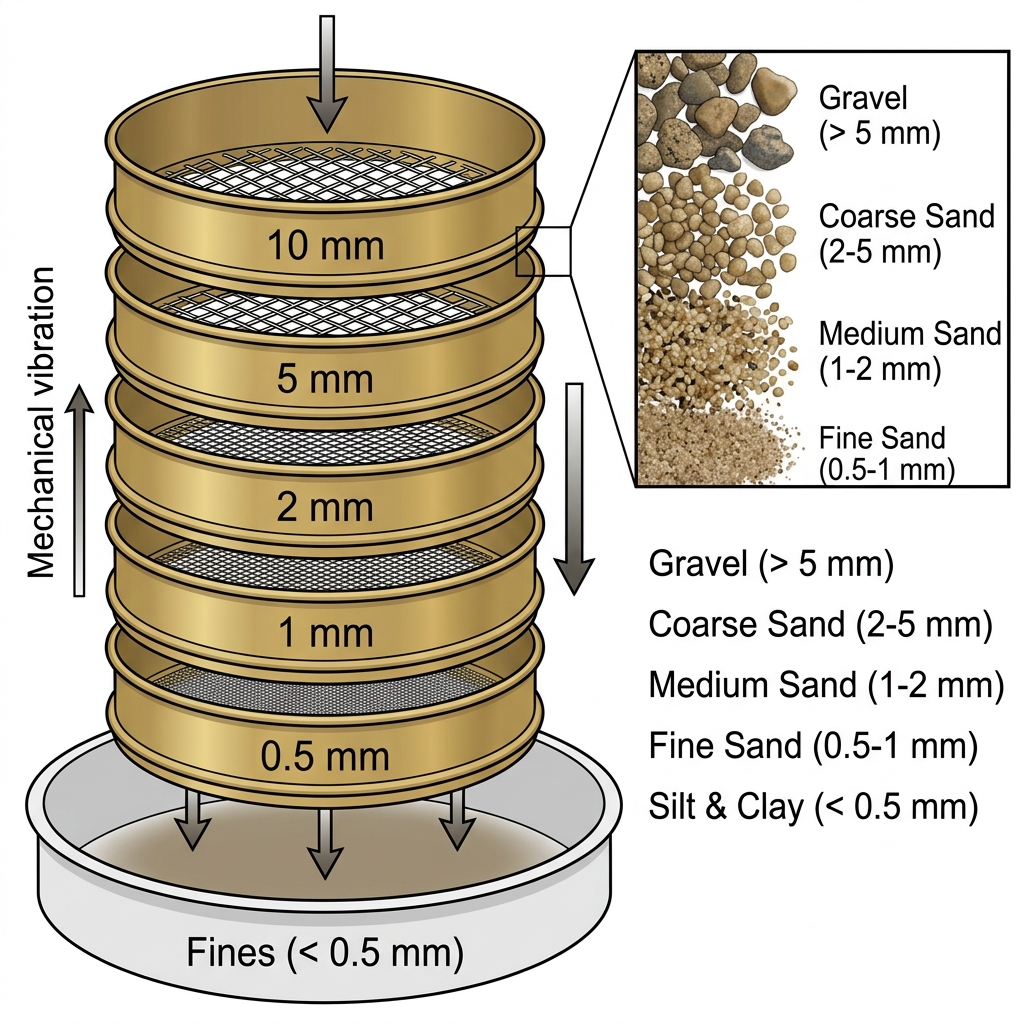
\includegraphics[width=\textwidth]{images/granulometrie.png}
        \caption{Séparation granulométrique}
    \end{subfigure}
    \hfill
    \begin{subfigure}[b]{0.32\textwidth}
        \centering
        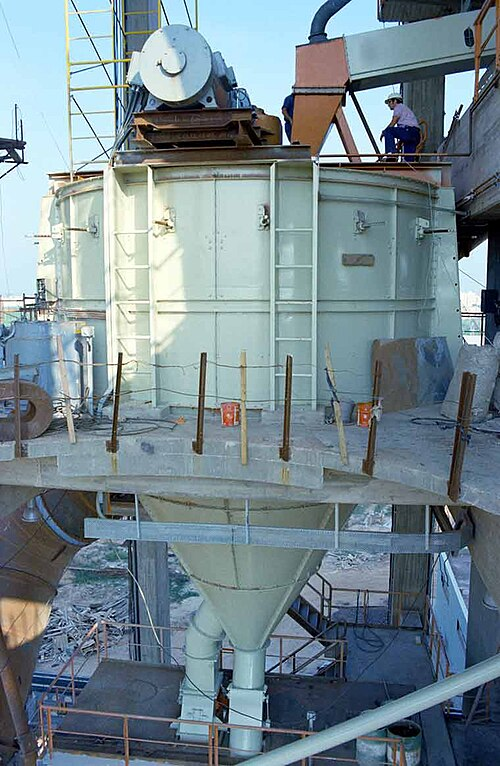
\includegraphics[width=\textwidth, height=4.5cm, keepaspectratio]{images/Zoubov-Sturtevant-whirlwind-centrifugal-Air-classifier-air-separator.jpg}
        \caption{Séparation aéraulique}
    \end{subfigure}
    \hfill
    \begin{subfigure}[b]{0.32\textwidth}
        \centering
        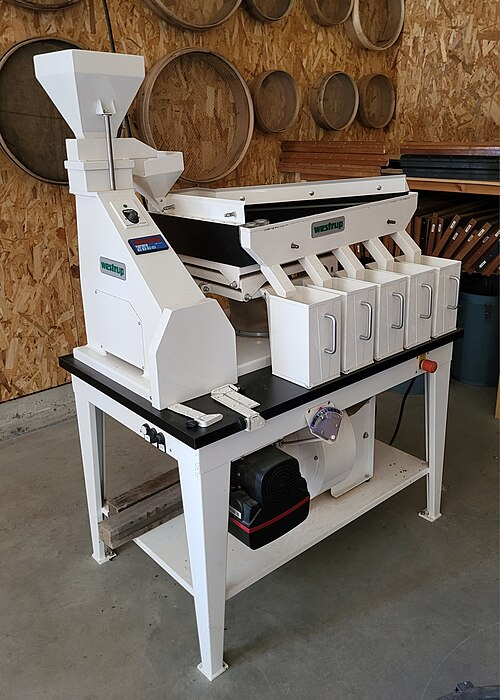
\includegraphics[width=\textwidth, height=4.5cm, keepaspectratio]{images/Table_densimétrique12.jpg}
        \caption{Séparation densimétrique}
    \end{subfigure}
    \caption{Principes physiques de triage des grains}
    \label{fig:tri_physique}
\end{figure}

\begin{itemize}
    \item \textbf{Séparation granulométrique :} Tamis vibrants ou rotatifs classant les grains selon leur taille et leur épaisseur (principe retenu pour le Bloc 2 de SMART-SOJA).
    \item \textbf{Séparation aéraulique :} Flux d'air vertical emportant les impuretés légères (poussières, gousses vides) tout en conservant les grains lourds.
    \item \textbf{Séparation densimétrique :} Table densimétrique exploitant un lit fluidisé pour trier des éléments de même taille mais de densités différentes.
\end{itemize}

\subsection{État de l'art industriel}
Au niveau industriel, les trieurs optiques représentent la solution la plus avancée : ils utilisent des caméras haute résolution et des algorithmes de traitement d'image pour éjecter les grains défectueux par jets d'air comprimé \cite{mahajan2015}. Bien que performants, leur coût élevé et leurs besoins énergétiques importants les rendent inaccessibles aux petits producteurs ruraux, justifiant une approche mécatronique plus abordable pour SMART-SOJA.

\begin{figure}[H]
    \centering
    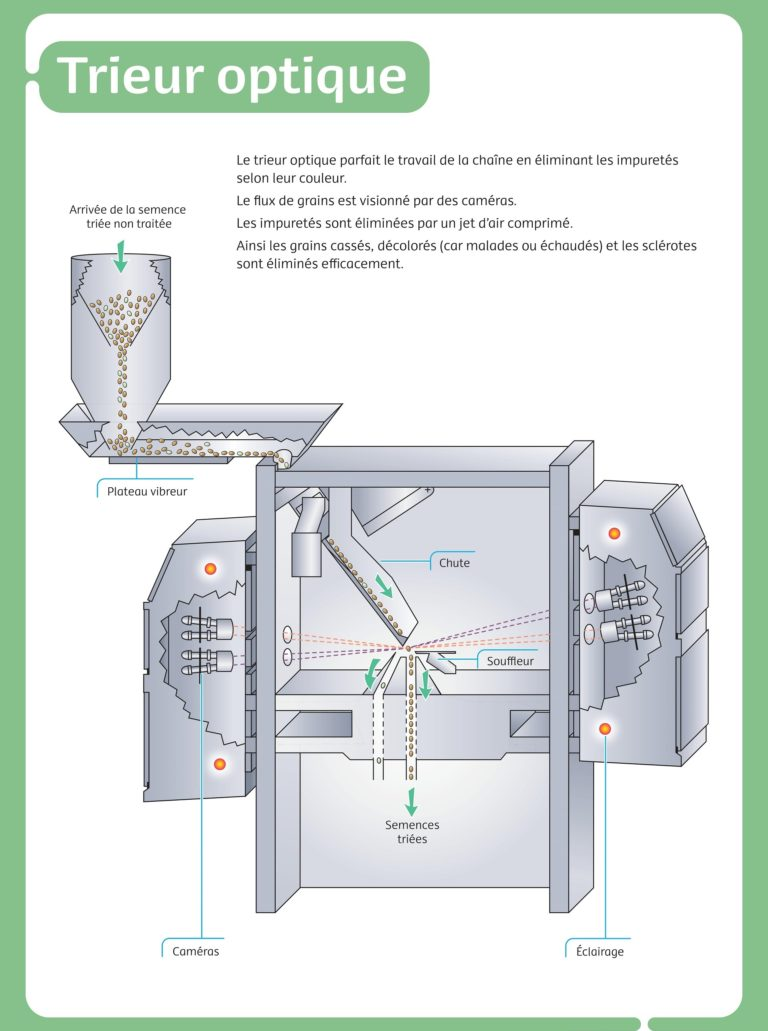
\includegraphics[height=6cm, keepaspectratio]{images/semae-pedagogie-station-semences-trieur-optique-768x1031.jpg}
    \caption{Exemple de trieur optique industriel haute résolution (Source : SEMAE Pédagogie)}
    \label{fig:trieur_optique}
\end{figure}

\FloatBarrier

% -------------------------------------------------------
\section{L'Internet des objets dans le secteur agricole (Agriculture 4.0)}
% -------------------------------------------------------

\subsection{Réseaux de capteurs sans fil (WSN) et connectivité LPWAN}
L'intégration de l'Internet des objets en agriculture (\textit{Smart Farming}) transforme la collecte et l'exploitation des données de terrain \cite{tarekegn2020}. Pour les zones rurales, les technologies \textbf{LPWAN} (\textit{Low-Power Wide-Area Network}) sont particulièrement adaptées en raison de leur longue portée et de leur faible consommation énergétique \cite{hanes2017, tzounis2017}.

\begin{figure}[H]
    \centering
    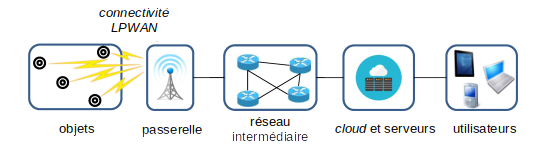
\includegraphics[width=0.65\textwidth]{images/Sensors-LPWAN.png}
    \caption{Architecture de connectivité LPWAN pour capteurs agricoles}
    \label{fig:iot_connectivity}
\end{figure}

Le protocole \textbf{MQTT} (\textit{Message Queuing Telemetry Transport}) constitue le standard de facto de l'Internet des objets industriel léger : son architecture Publication/Abonnement permet une communication robuste sur des réseaux à bande passante limitée et connexion instable, comme les zones rurales du Bénin \cite{mqtt_org, hanes2017}.

\subsection{Traçabilité numérique et Big Data agricole}
La numérisation des données de qualité crée un \textit{passeport numérique} du grain depuis le champ jusqu'à l'usine. Les travaux de recherche montrent que la structuration de ces données en format \textbf{JSON} permet de limiter les fraudes, de garantir les standards qualité de la GDIZ et d'ouvrir la voie à des analyses prédictives (Big Data agricole) pour l'amélioration continue des processus.


\subsection{Autonomie énergétique en milieu rural}
L'électrification rurale étant défaillante dans de nombreuses zones de production, la littérature technique privilégie les systèmes photovoltaïques hybrides avec régulateurs \textbf{MPPT} (\textit{Maximum Power Point Tracking}) pour optimiser l'extraction d'énergie solaire, abondante dans les régions tropicales comme le Bénin.

\FloatBarrier

% -------------------------------------------------------
\section{Cahier des charges fonctionnel}
% -------------------------------------------------------

L'analyse du contexte de la filière soja, des exigences normatives (NB~01.07.004) et des limites des solutions existantes permet de formuler le cahier des charges fonctionnel du système SMART-SOJA. Ce document de référence définit les fonctions que le prototype doit remplir, les critères d'acceptation et les moyens de validation associés. Les fonctions sont classées en \textbf{fonctions principales} (FP), directement liées aux objectifs du système, et en \textbf{fonctions contraintes} (FC), imposées par l'environnement d'utilisation.

\subsection{Fonctions principales}

Le Tableau~\ref{tab:cdc_fp} détaille les sept fonctions principales du système, issues des objectifs spécifiques du mémoire et des exigences de la norme \textbf{NB~01.07.004}.

\begin{table}[H]
    \caption{Cahier des charges fonctionnel — Fonctions principales (FP)}
    \label{tab:cdc_fp}
    \centering
\footnotesize
\renewcommand{\arraystretch}{1.5}
\rowcolors{2}{white}{lightGray}
\begin{tabularx}{\textwidth}{|p{2.3cm}|L|p{2.1cm}|L|L|}
\hline
\rowcolor{lightGray}
\textbf{Fonction} & \textbf{Exigence} & \textbf{Valeur cible} & \textbf{Justification} & \textbf{Moyen de vérification} \\ \hline

\textbf{FP1}\newline Nettoyage &
Séparer les impuretés des grains par tamisage vibrant &
Pureté $>$ 98~\% &
Norme NB~01.07.004, exigence GDIZ &
Pesée différentielle avant/après, inspection visuelle \\ \hline

\textbf{FP2}\newline Mesure humidité &
Mesurer le taux d'humidité en deux points du lot (Soil1/Soil2) &
$\pm\,5$~\% HR, seuil 12~\% &
Norme NB~01.07.004 &
Comparaison avec hygromètre de référence certifié \\ \hline

\textbf{FP3}\newline Séchage actif &
Réduire l'humidité par air chaud et brassage si $H > 12$~\% &
$H \leq 12$~\% en sortie (double validation) &
Prévention moisissures, conformité GDIZ &
Lecture convergente Soil1 ET Soil2 $\leq$ 12~\% \\ \hline

\textbf{FP4}\newline Pesée &
Peser chaque lot traité avec précision &
0--10~kg, $\pm\,0{,}1$~\% &
Certification du poids pour traçabilité &
Étalonnage poids de référence (module HX711) \\ \hline

\textbf{FP5}\newline Traçabilité IoT &
Générer un passeport numérique JSON par lot et le transmettre via MQTT &
Payload JSON complet, publication MQTT &
Transparence et fiabilité de la chaîne d'approvisionnement &
Réception et décodage sur broker HiveMQ \\ \hline

\textbf{FP6}\newline Autonomie &
Fonctionner en autonomie solaire hors réseau électrique &
$\geq$ 3~h/jour, recharge solaire en 5~h &
Zones rurales non électrifiées &
Mesure tension batterie, durée de cycle effective \\ \hline

\textbf{FP7}\newline Mobilité &
Déplacer l'unité vers les sites de collecte &
Châssis sur roulettes, compatible véhicule utilitaire &
Rapprocher la technologie du producteur &
Test de déplacement sur terrain plat et piste \\ \hline

\end{tabularx}
\end{table}

\subsection{Fonctions contraintes}

Le Tableau~\ref{tab:cdc_fc} regroupe les contraintes imposées par l'environnement opérationnel, la sécurité et la maintenabilité du système.

\begin{table}[H]
    \caption{Cahier des charges fonctionnel — Fonctions contraintes (FC)}
    \label{tab:cdc_fc}
    \centering
\footnotesize
\renewcommand{\arraystretch}{1.5}
\rowcolors{2}{white}{lightGray}
\begin{tabularx}{\textwidth}{|p{2.3cm}|L|p{2.1cm}|L|L|}
\hline
\rowcolor{lightGray}
\textbf{Fonction} & \textbf{Exigence} & \textbf{Valeur cible} & \textbf{Justification} & \textbf{Moyen de vérification} \\ \hline

\textbf{FC1}\newline Interface opérateur &
Affichage et contrôle local du cycle &
LCD 16$\times$2, 2 potentiomètres, boutons, LEDs &
Opérateur non expert en milieu rural &
Test d'utilisabilité en conditions réelles \\ \hline

\textbf{FC2}\newline Contrôle temps réel &
Automatisation séquentielle (GRAFCET) avec sécurité prioritaire &
Temps de réponse sécurité $<$ 10~ms &
Sûreté de fonctionnement, arrêt d'urgence &
Test arrêt d'urgence, chronogramme FreeRTOS \\ \hline

\textbf{FC3}\newline Résilience réseau &
Aucune perte de données en l'absence de WiFi &
\textit{Store-and-Forward} sur carte MicroSD &
Couverture WiFi limitée en zone rurale &
Test déconnexion/reconnexion, intégrité données \\ \hline

\textbf{FC4}\newline Maintenabilité &
Accès individuel aux sous-systèmes sans démontage intégral &
4 blocs amovibles, connecteurs rapides &
Maintenance en milieu rural isolé &
Démontage et remontage d'un bloc $<$ 15~min \\ \hline

\textbf{FC5}\newline Robustesse &
Résistance aux vibrations, poussière et chocs de transport &
Châssis acier 40~mm, tamis inox 304, roulettes caoutchouc &
Usage en extérieur, transport sur pistes &
Inspection visuelle après campagne de tests \\ \hline

\textbf{FC6}\newline Coût &
Accessibilité financière du prototype &
Composants standard, disponibles localement &
Cible : coopératives et petits producteurs &
Bilan financier détaillé des composants \\ \hline

\end{tabularx}
\end{table}

Ce cahier des charges constitue le document de référence pour la suite de l'étude. Chaque fonction sera traitée dans les sections suivantes à travers les choix d'architecture, de composants et de dimensionnement du système SMART-SOJA.

% Fin de la section contexte


% -------------------------------------------------------
% PARTIE 2 : MATÉRIELS ET MÉTHODES
% -------------------------------------------------------

% ---- SECTION MATÉRIELS ET MÉTHODES ----

% -------------------------------------------------------
\section{Architecture système globale}
% -------------------------------------------------------
Le système \textbf{SMART-SOJA} repose sur une architecture modulaire et hiérarchisée structurée en trois couches fonctionnelles (Figure \ref{fig:architecture_complete}) :

\begin{figure}[H]
    \centering
    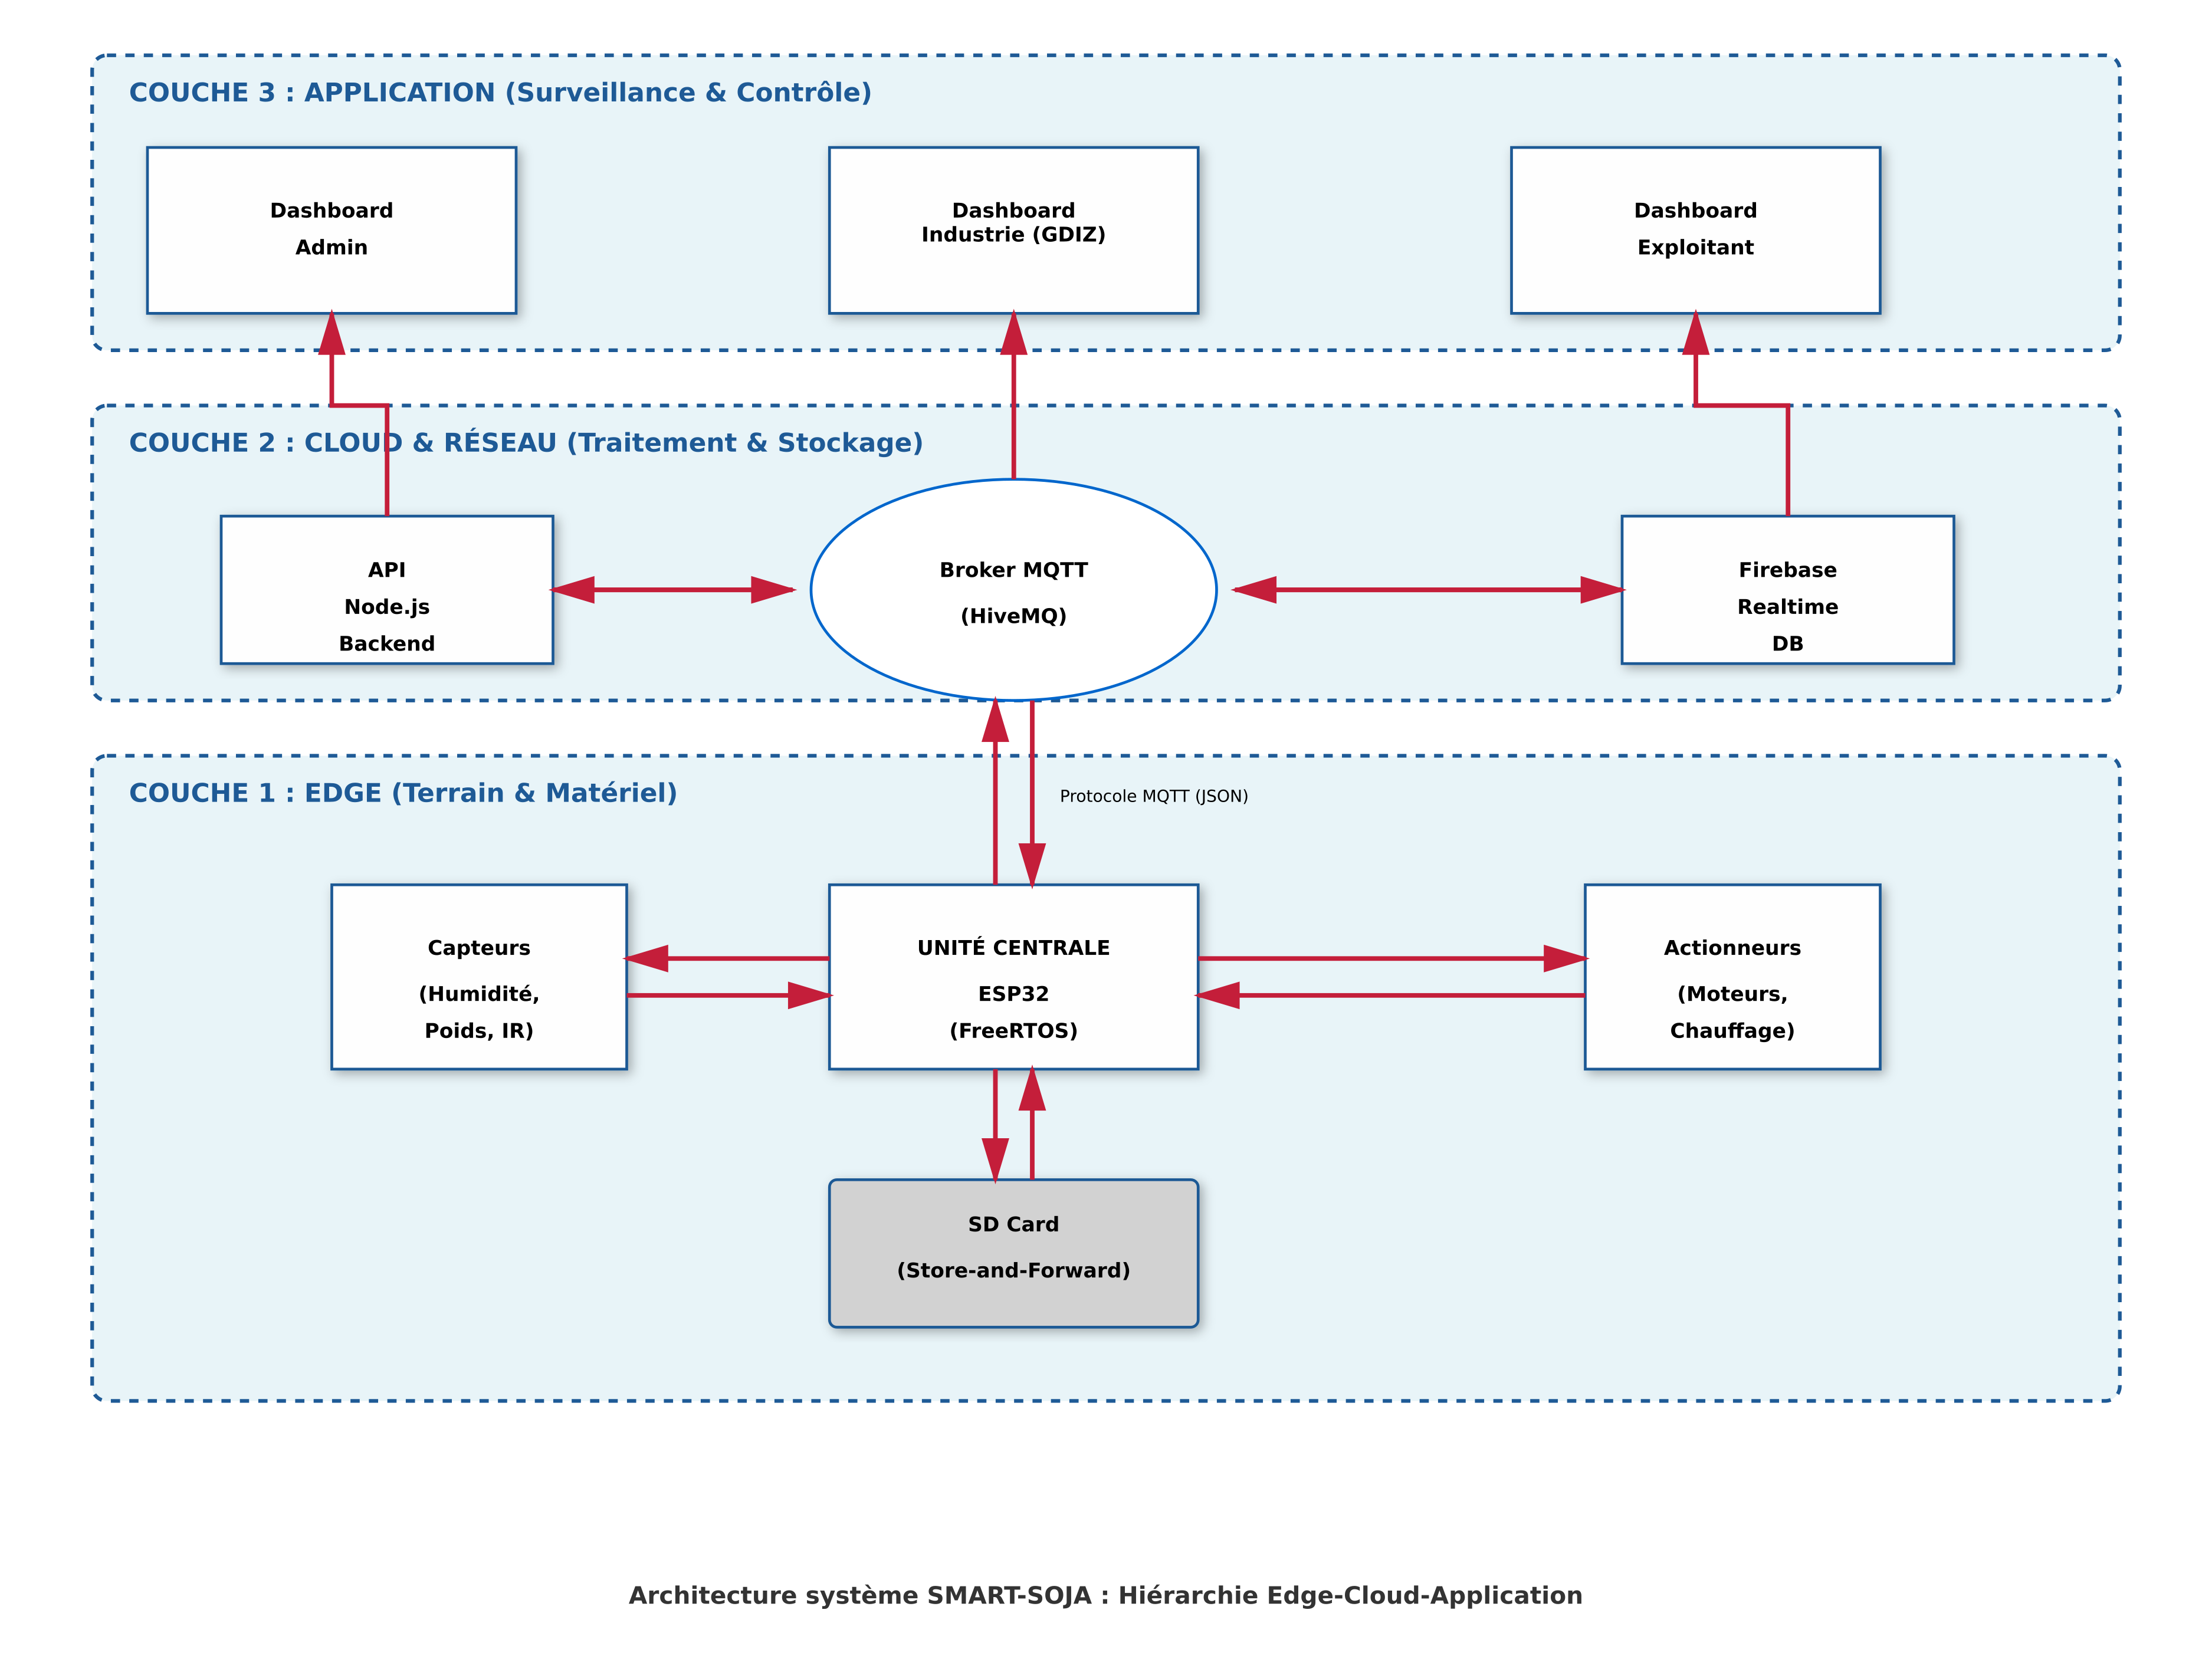
\includegraphics[width=\textwidth]{images/architecture_smart_soja.png}
    \caption{Architecture système SMART-SOJA : Hiérarchie Edge-Cloud-Application}
    \label{fig:architecture_complete}
\end{figure}
\FloatBarrier

\begin{itemize}
    \item \textbf{Couche Edge (Terrain) :} L'ESP32 gère en temps réel l'acquisition des capteurs, le pilotage des actionneurs et la logique de contrôle GRAFCET.
    \item \textbf{Couche Cloud :} Un broker MQTT (HiveMQ) relié à une API Node.js et une base Firebase assure le stockage et le traitement des données de traçabilité.
    \item \textbf{Couche Application :} Des tableaux de bord web (rôles Admin, Industrie, Exploitant) permettent le suivi à distance de chaque lot traité.
\end{itemize}

Cette architecture (Figure \ref{fig:architecture_complete}) garantit un fonctionnement autonome complet en mode déconnecté (\textit{Store-and-Forward} sur carte SD), tout en s'intégrant nativement dans une infrastructure Cloud de type Industrie 4.0. Elle permet une résilience face aux pannes de réseau fréquentes en milieu rural tout en assurant une visibilité globale pour les unités de transformation.

% -------------------------------------------------------
\section{Sous-système électronique et informatique}
% -------------------------------------------------------

\subsection{Unité de traitement : l'ESP32-WROOM-32}

Le microcontrôleur \textbf{ESP32-WROOM-32} (Figure \ref{fig:esp32_presentation}) constitue le cœur décisionnel du système \cite{esp32_datasheet}. Ses spécifications techniques sont résumées dans le Tableau \ref{tab:specs_esp32}.

\begin{table}[H]
    \caption{Spécifications techniques du microcontrôleur ESP32-WROOM-32}
    \label{tab:specs_esp32}
    \centering
    \small
    \renewcommand{\arraystretch}{1.4}
    \rowcolors{2}{white}{lightGray}
    \begin{tabularx}{\textwidth}{|L|>{\bfseries}L|}
        \hline
        \rowcolor{lightGray}
        \textbf{Caractéristique} & \textbf{Spécification} \\ \hline
        Microcontrôleur & Tensilica LX6 double cœur 240 MHz \\ \hline
        Alimentation & 5~V DC (microUSB) / 3,3~V DC (E/S) \\ \hline
        Consommation veille & 5~\textmu A (Ultra-low power) \\ \hline
        Mémoire & 520 Ko SRAM / 4 Mo Flash \\ \hline
        Connectivité & Wi-Fi 802.11 b/g/n + Bluetooth 4.2 \\ \hline
        GPIO & 30 broches (3x UART, 2x I2C, 3x SPI, 12x ADC, 2x DAC) \\ \hline
        Dimensions & 55 × 28 × 8 mm / 11 g \\ \hline
    \end{tabularx}
\end{table}

\begin{figure}[H]
    \centering
    \begin{subfigure}[b]{0.45\textwidth}
        \centering
        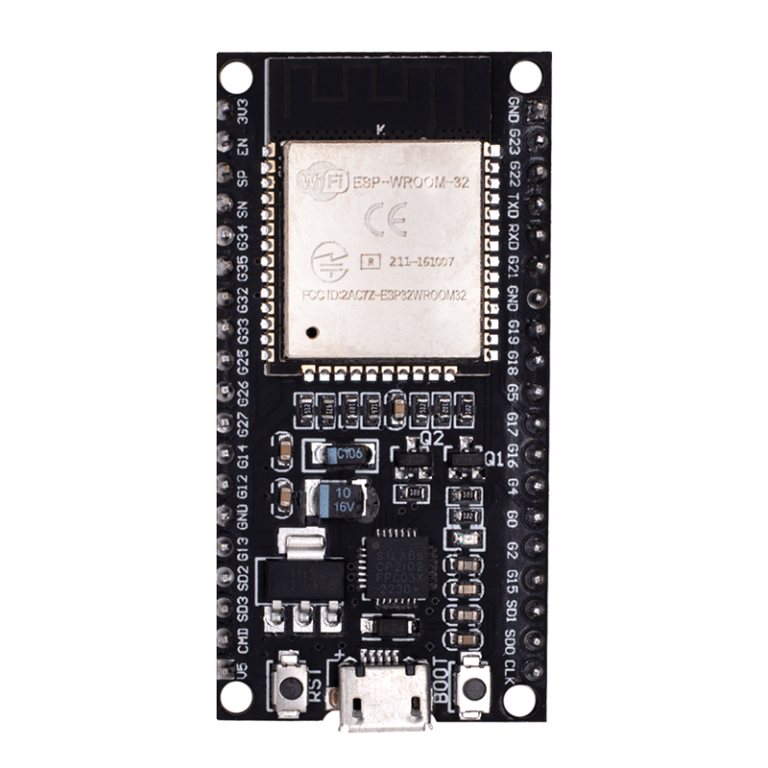
\includegraphics[width=\textwidth]{images/image_esp32.png}
        \caption{Module ESP32-WROOM-32}
    \end{subfigure}
    \hfill
    \begin{subfigure}[b]{0.45\textwidth}
        \centering
        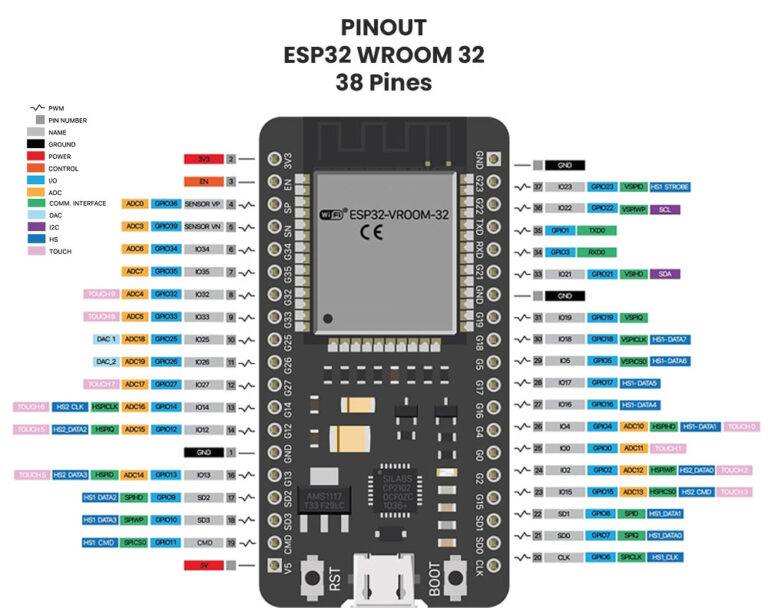
\includegraphics[width=\textwidth]{images/pinout_esp32.jpg}
        \caption{Brochage (Pinout)}
    \end{subfigure}
    \caption{Présentation du microcontrôleur ESP32}
    \label{fig:esp32_presentation}
\end{figure}
\FloatBarrier

\textbf{Justification du choix :} L'architecture Dual-Core permet de dédier un cœur au contrôle-commande temps réel (capteurs, actionneurs PWM) et l'autre à la communication Internet des objets (MQTT/WiFi), garantissant un déterminisme critique. La consommation de 5~\textmu A en veille optimise l'autonomie solaire, et les 30 GPIO offrent la flexibilité nécessaire pour tous les bus I2C, SPI et interfaces ADC du système.

\subsection{Chaîne d'acquisition : les capteurs}

Quatre capteurs stratégiques (Figure \ref{fig:capteurs_systeme}) assurent le suivi de la qualité et le déclenchement automatique des actions du GRAFCET (Tableau \ref{tab:specs_capteurs}).

\begin{table}[H]
    \caption{Spécifications détaillées de la chaîne d'acquisition}
    \label{tab:specs_capteurs}
    \centering
    \small
    \renewcommand{\arraystretch}{1.5}
    \rowcolors{2}{white}{lightGray}
    \begin{tabularx}{\textwidth}{|L|C|C|L|L|}
        \hline
        \rowcolor{lightGray}
        \textbf{Capteur} & \textbf{Plage / Précision} & \textbf{Calibration} & \textbf{Rôle} & \textbf{Limites} \\ \hline
        DHT22 & 0-100\% RH / ±2\% & Usine (1-Wire) & Humidité/Temp. ambiante & Temps réponse 2s \\ \hline
        Sonde Capacitive & 0-100\% (HR equiv.) / ±5\% & In-situ (soja sec/humide) & Humidité grains (Soil1, Soil2) & Dérive thermique \\ \hline
        IR Réflectif & 2-30 cm / Binaire & Trimpot manuel & Présence trémie/sac & Lumière ambiante \\ \hline
        Cellule de charge & 0-10 kg / ±0,1\% & Poids étalon (HX711) & Pesée finale du lot & Vibrations mécaniques \\ \hline
    \end{tabularx}
\end{table}

\begin{figure}[H]
    \centering
    \begin{subfigure}[b]{0.22\textwidth}
        \centering
        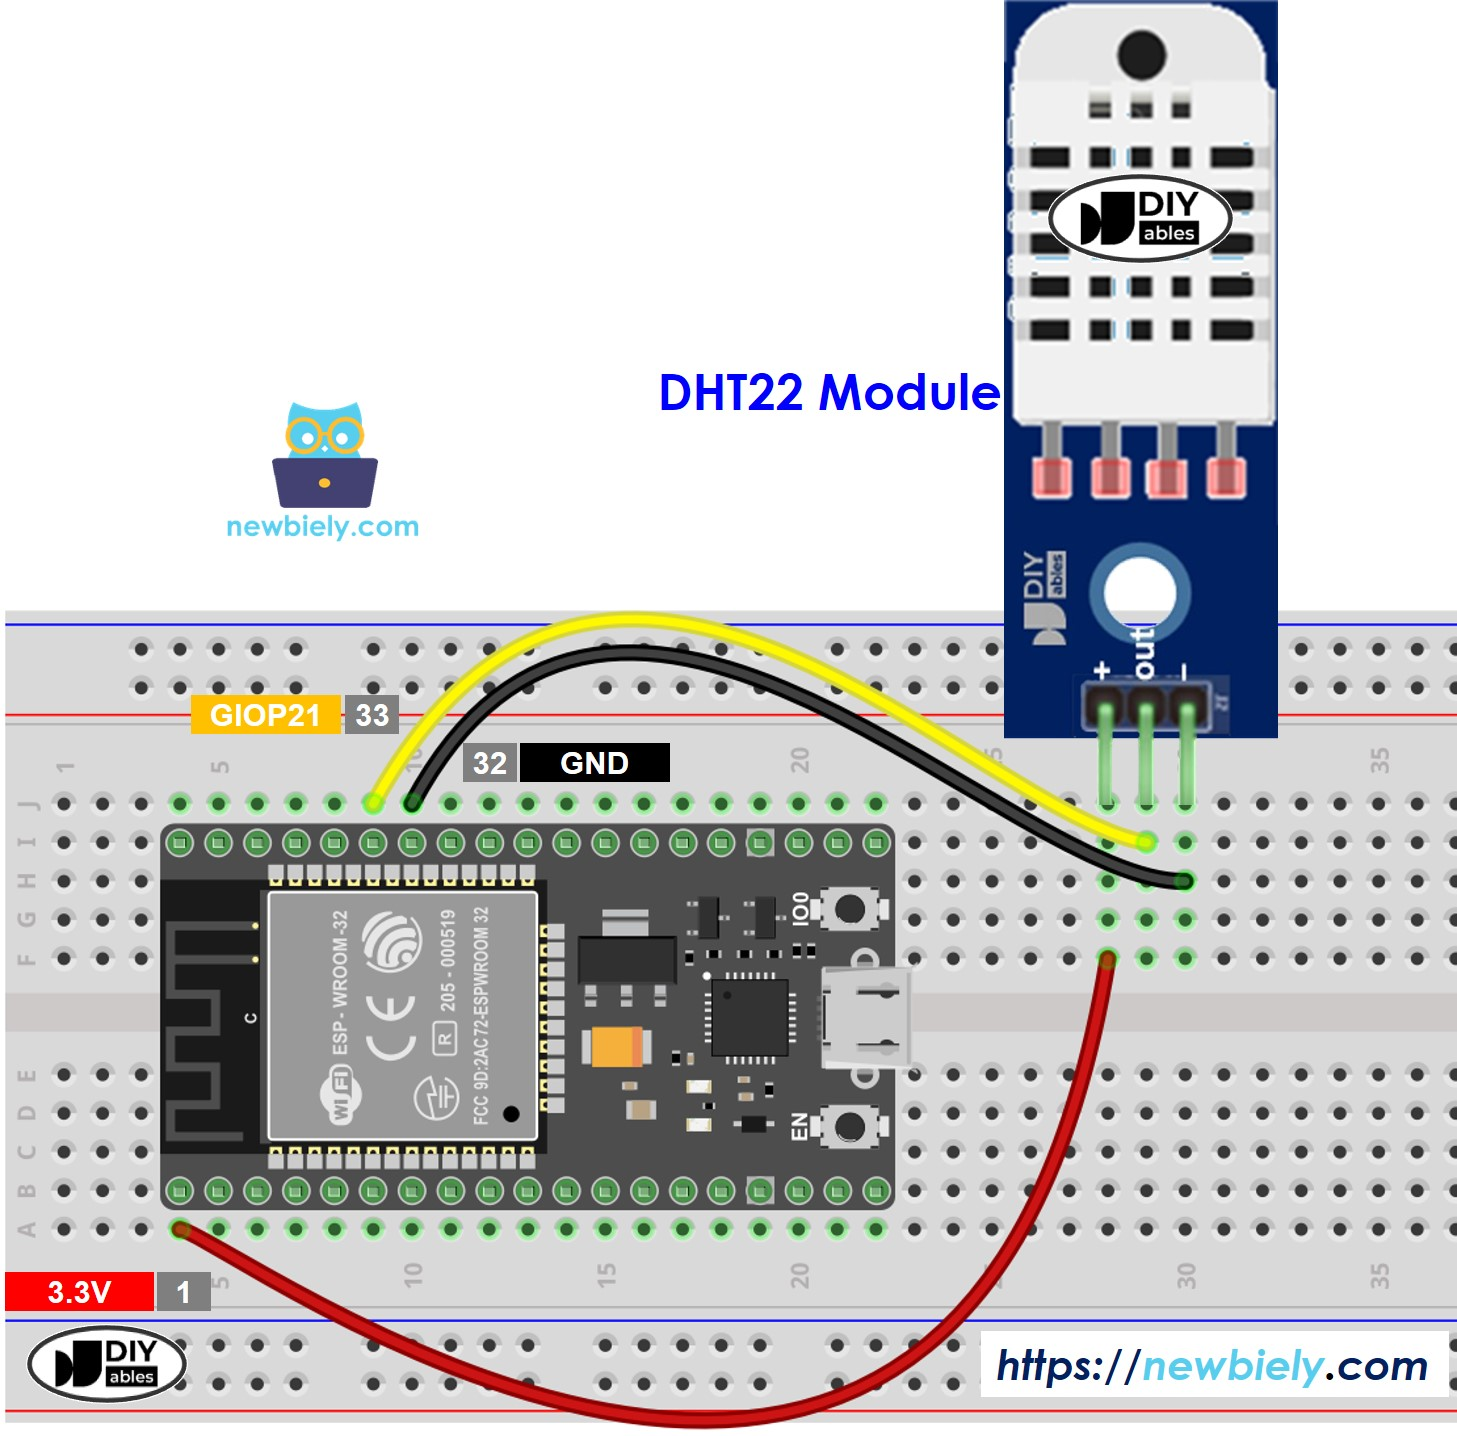
\includegraphics[width=\textwidth]{images/esp32-dht22-module-broche3.jpg}
        \caption{DHT22}
    \end{subfigure}
    \hfill
    \begin{subfigure}[b]{0.22\textwidth}
        \centering
        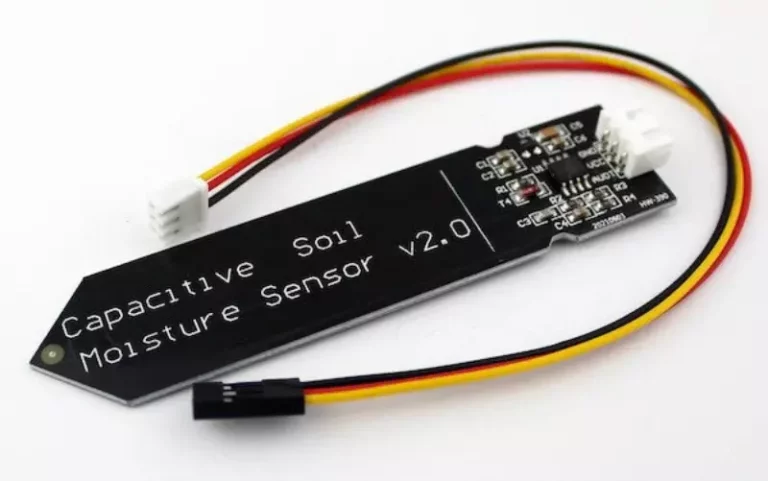
\includegraphics[width=\textwidth]{images/Capacitive-Soil-Moisture-Sensor-768x481.png}
        \caption{Sonde capacitive}
    \end{subfigure}
    \hfill
    \begin{subfigure}[b]{0.22\textwidth}
        \centering
        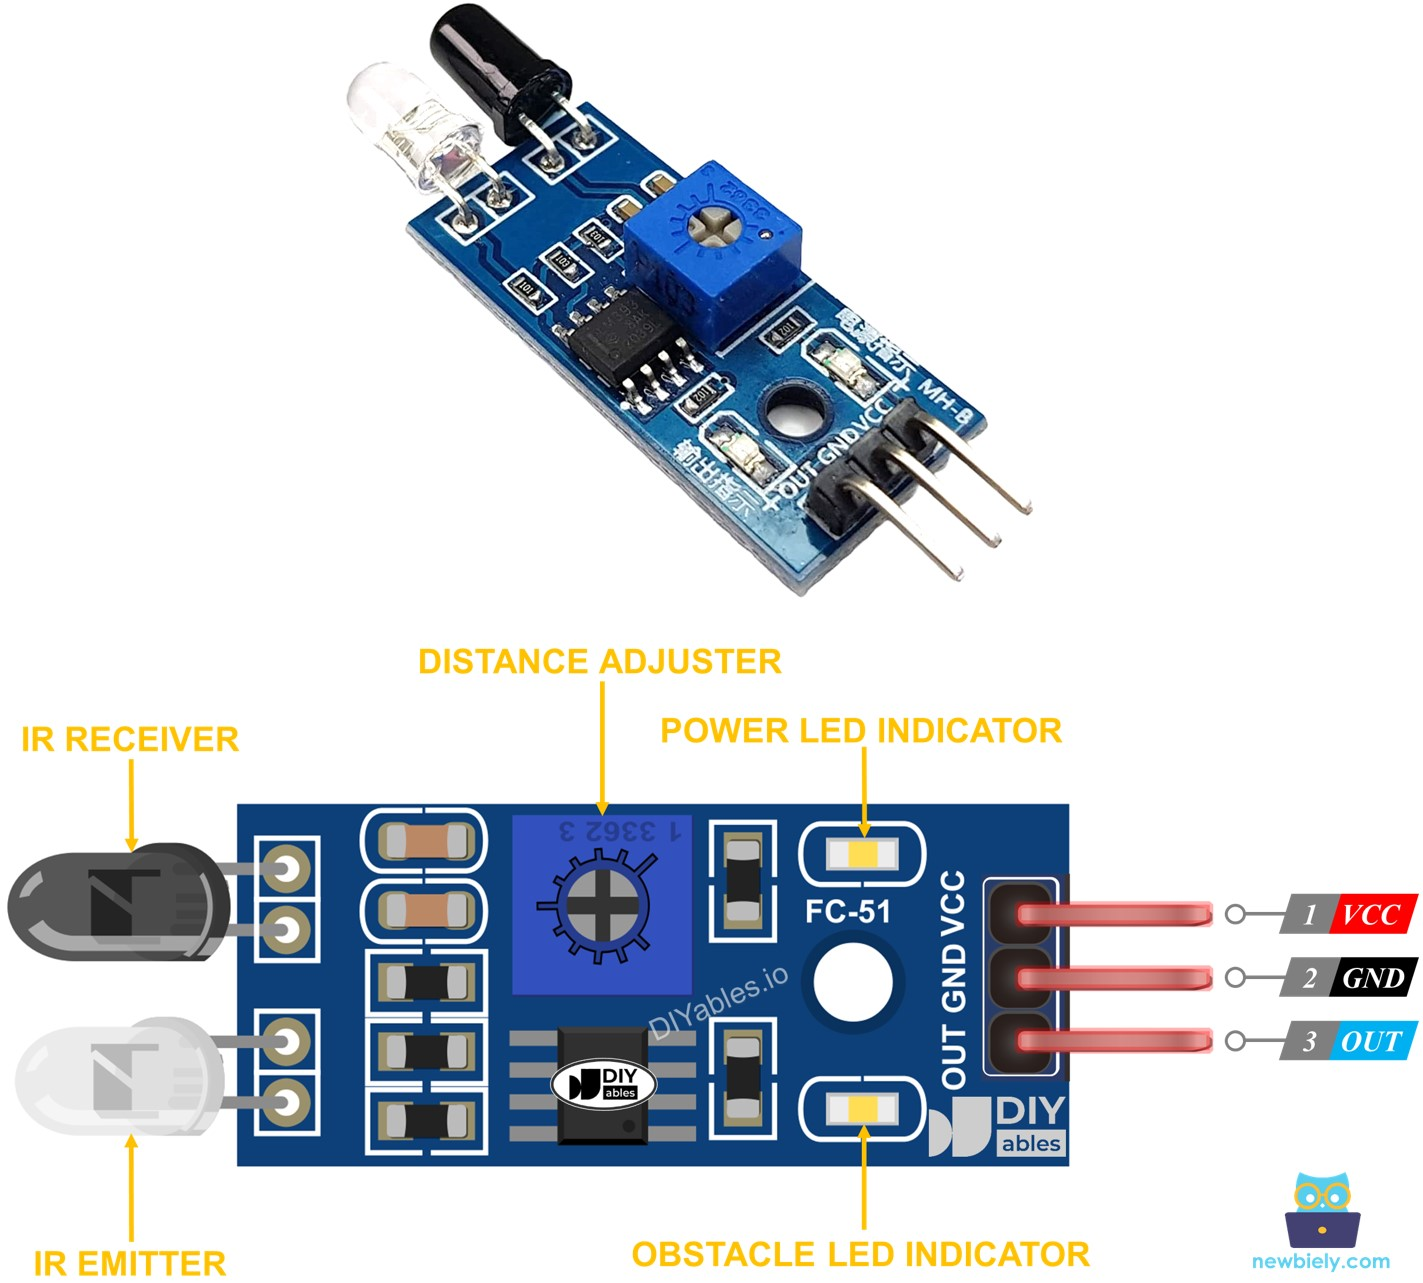
\includegraphics[width=\textwidth]{images/IR-avoidance-sensor-pinout.jpg}
        \caption{Capteur IR}
    \end{subfigure}
    \hfill
    \begin{subfigure}[b]{0.22\textwidth}
        \centering
        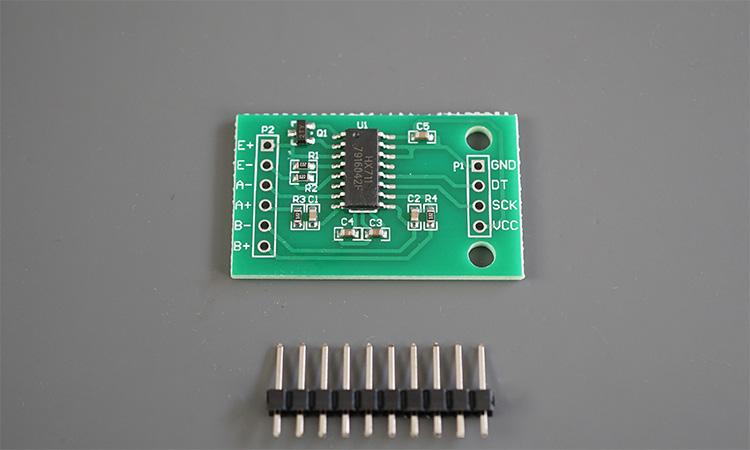
\includegraphics[width=\textwidth]{images/hx711-amplifier.jpg}
        \caption{Module HX711}
    \end{subfigure}
    \caption{Capteurs intégrés au système SMART-SOJA}
    \label{fig:capteurs_systeme}
\end{figure}
L'intégration de cette chaîne d'acquisition (Figure \ref{fig:capteurs_systeme}) permet de couvrir l'intégralité des besoins de suivi : l'humidité ambiante influe sur la cinétique de séchage, les sondes capacitives valident la qualité intrinsèque, l'infrarouge gère l'automatisation du flux et la cellule de charge certifie le poids final.

La \textbf{sonde d'humidité capacitive} mérite une attention particulière : elle mesure la constante diélectrique du milieu (eau $\approx$ 80 vs. grain sec $\approx$ 3--5), ce qui la rend insensible à la corrosion — avantage décisif pour un usage en contact direct avec les grains de soja. Deux sondes (Soil1 et Soil2) sont positionnées respectivement en haut et en bas de la zone de séchage, permettant un calcul d'humidité moyenne en deux points.

\textbf{Calibration in-situ :} La sonde capacitive délivre une tension analogique lue par le convertisseur ADC 12 bits de l'ESP32 (plage 0--4095). Une calibration en deux points est réalisée avant chaque campagne d'essai :
\begin{enumerate}
    \item \textbf{Point sec} ($H \approx 8~\%$) : un échantillon de soja séché à l'étuve est placé autour de la sonde ; la valeur ADC correspondante est enregistrée comme borne haute (soja conforme).
    \item \textbf{Point humide} ($H \approx 20~\%$) : un échantillon saturé en humidité sert de borne basse (soja non conforme).
\end{enumerate}
Une interpolation linéaire entre ces deux bornes permet de convertir toute lecture ADC intermédiaire en un taux d'humidité exprimé en pourcentage. Cette méthode simple mais robuste est validée par comparaison avec les mesures de l'hygromètre de référence Testo 608-H2, avec un écart maximal observé de $\pm 5~\%$ conformément à la spécification du capteur (Tableau~\ref{tab:specs_capteurs}).

\subsection{Chaîne d'action : actionneurs et interface de puissance}

Le pilotage des charges électromécaniques (12~V, forts courants) depuis un microcontrôleur 3,3~V nécessite des interfaces de puissance adaptées (Figure \ref{fig:actionneurs_systeme}). Le Tableau \ref{tab:specs_actionneurs} récapitule les actionneurs du système.

\begin{table}[H]
    \caption{Spécifications détaillées de la chaîne d'action}
    \label{tab:specs_actionneurs}
    \centering
    \small
    \renewcommand{\arraystretch}{1.5}
    \rowcolors{2}{white}{lightGray}
    \begin{tabularx}{\textwidth}{|L|C|L|L|}
        \hline
        \rowcolor{lightGray}
        \textbf{Actionneur} & \textbf{Puissance / Courant} & \textbf{Critère de dimensionnement} & \textbf{Protections} \\ \hline
        Moteurs JGA25 & 3~W / 0,5~A (max 1,2~A) & Couple de rotation pour tamis et vis & Diode roue libre \\ \hline
        MOSFET IRLZ44N & 175~W / 47~A (max) & Compatibilité \textit{Logic Level} (3,3~V) & Résistance de Gate \\ \hline
        Servo SG90 & 1,5~W / 0,1~A à 0,5~A & Couple de 1,3 kg.cm pour la vanne & Condensateur de filtrage \\ \hline
        Résistance & 12~W / 1~A & Delta Température pour séchage & Fusible thermique \\ \hline
        Ventilateur DC & 1,8~W / 0,15~A & Flux d'air de 15 CFM pour extraction & Diode roue libre \\ \hline
    \end{tabularx}
\end{table}

\begin{figure}[H]
    \centering
    \begin{subfigure}[b]{0.19\textwidth}
        \centering
        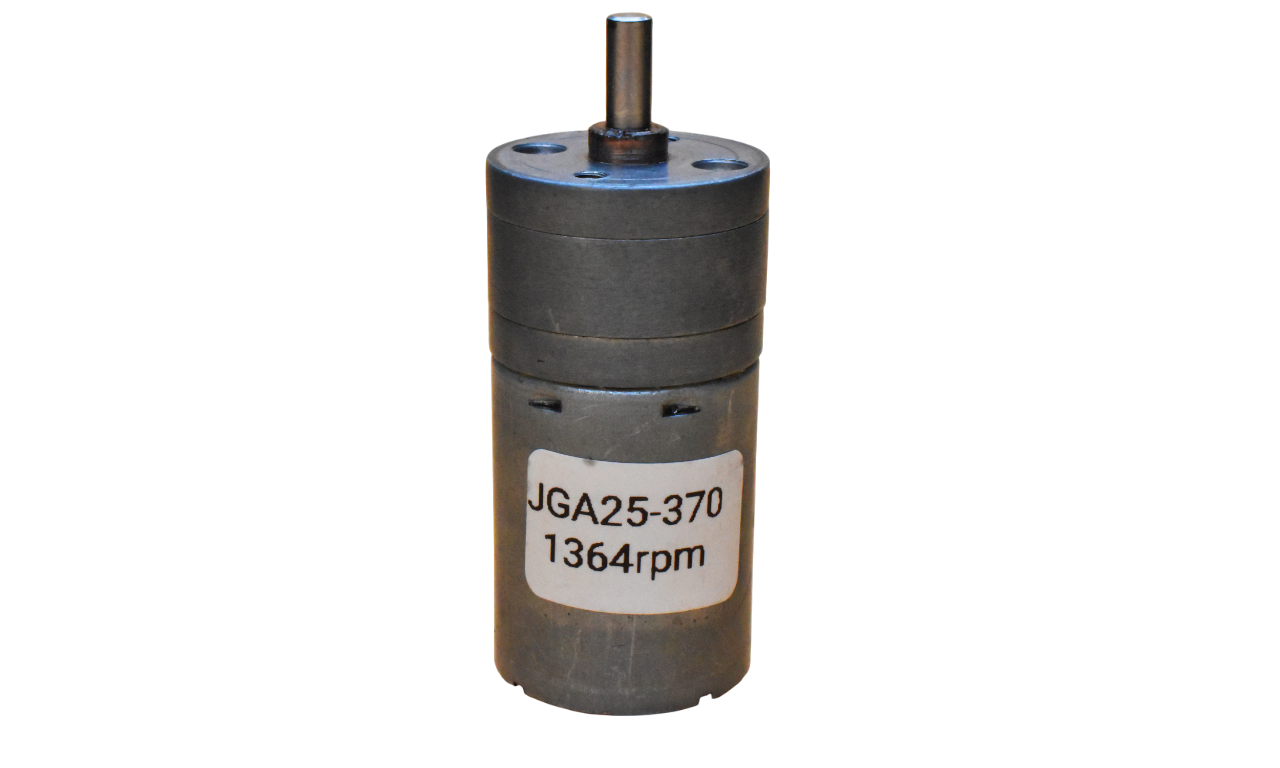
\includegraphics[width=\textwidth]{images/moteur_jga25-370 1364.png}
        \caption{Moteur JGA25}
    \end{subfigure}
    \hfill
    \begin{subfigure}[b]{0.19\textwidth}
        \centering
        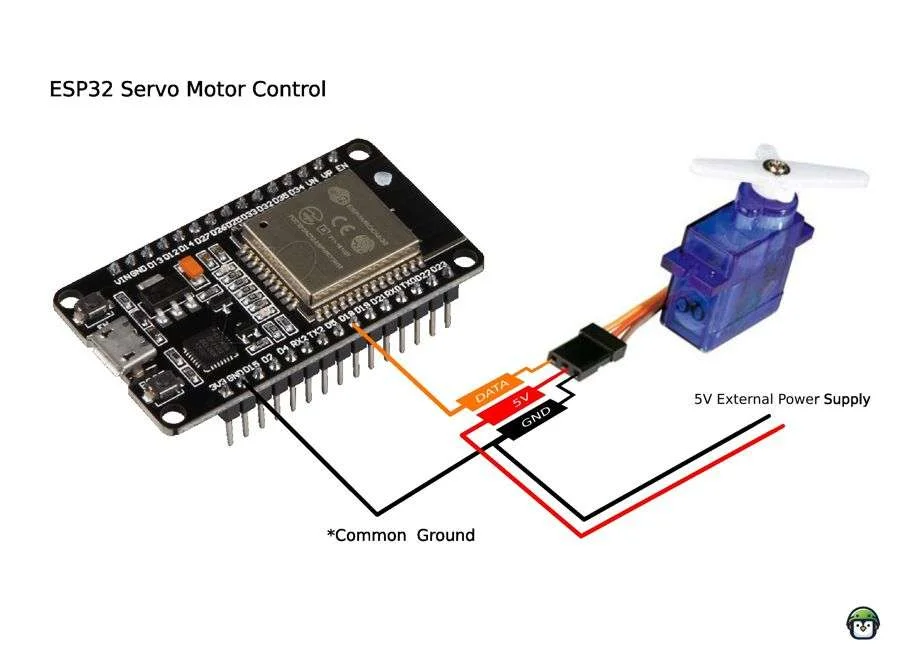
\includegraphics[width=\textwidth]{images/samgalope.dev-devdigest-ESP32-SERVO-SG90.png}
        \caption{Servo SG90}
    \end{subfigure}
    \hfill
    \begin{subfigure}[b]{0.19\textwidth}
        \centering
        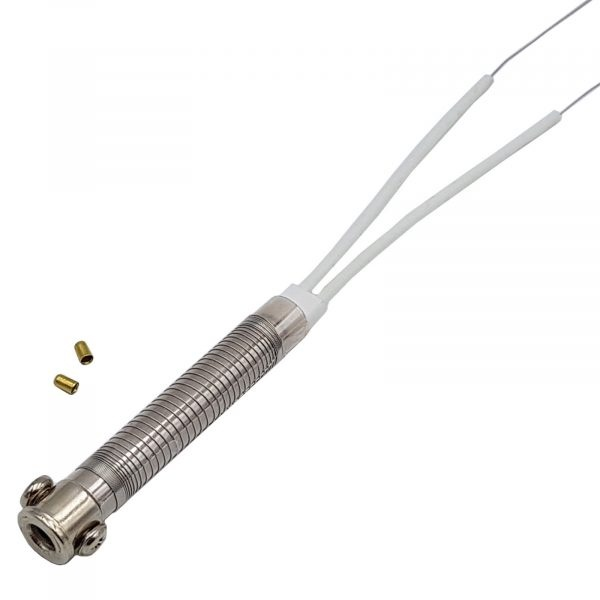
\includegraphics[width=\textwidth]{images/resistance_chauffante.jpg}
        \caption{Résistance}
    \end{subfigure}
    \hfill
    \begin{subfigure}[b]{0.19\textwidth}
        \centering
        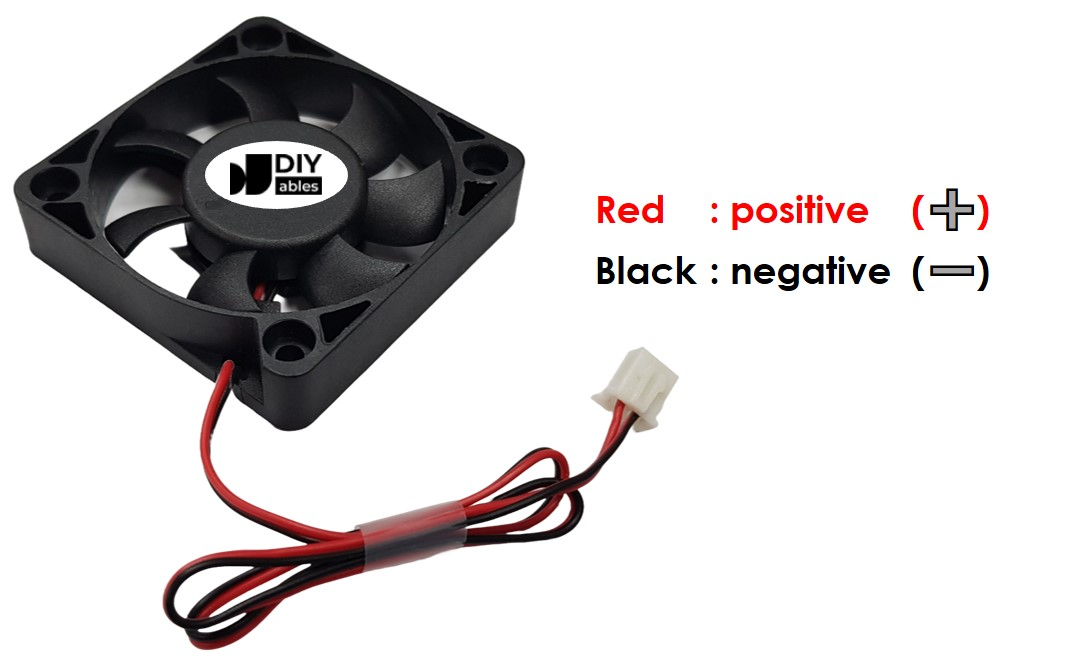
\includegraphics[width=\textwidth]{images/fan-pinout.jpg}
        \caption{Ventilateur}
    \end{subfigure}
    \hfill
    \begin{subfigure}[b]{0.19\textwidth}
        \centering
        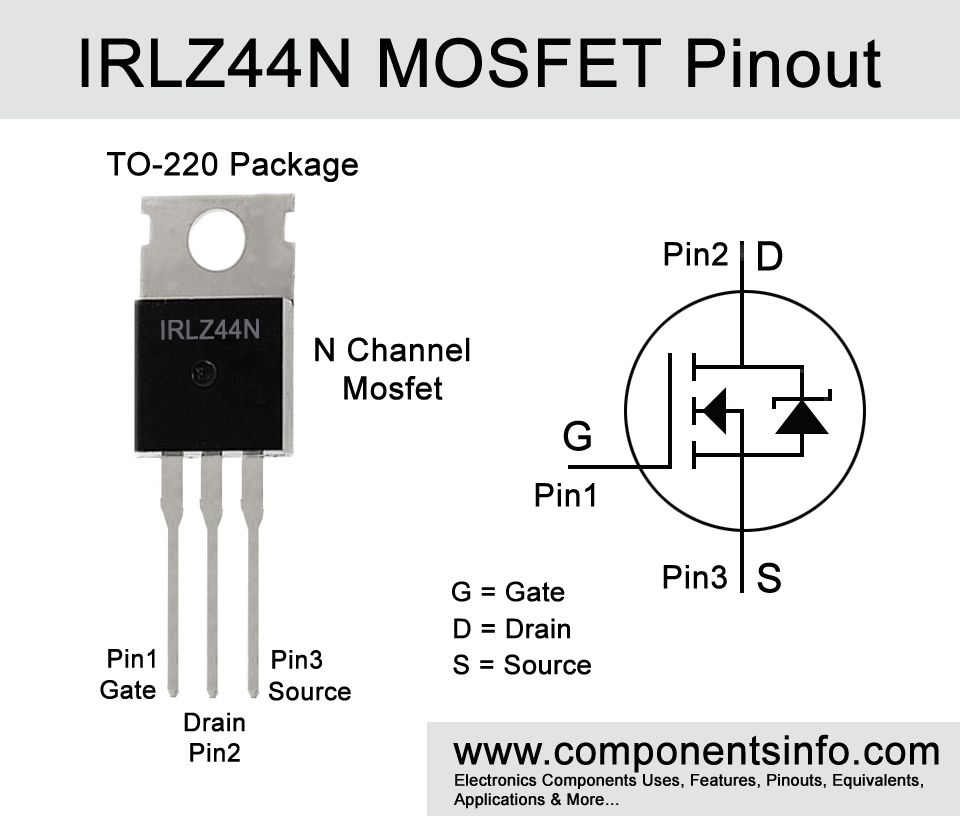
\includegraphics[width=\textwidth]{images/irlz44n-pinout-equivalent.png}
        \caption{MOSFET}
    \end{subfigure}
    \caption{Actionneurs et interface de puissance du système}
    \label{fig:actionneurs_systeme}
\end{figure}
\FloatBarrier

Le \textbf{MOSFET IRLZ44N} est retenu car, contrairement aux MOSFET standards nécessitant 10~V de commande, ce modèle \textit{Logic Level} se sature directement avec les 3,3~V de l'ESP32. Il peut commuter jusqu'à 47~A avec une résistance interne de seulement 0,022~$\Omega$, permettant un pilotage PWM précis des moteurs et de la résistance chauffante sans échauffement excessif \cite{irlz44n_datasheet}. Il convient de noter que la valeur de 175~W indiquée dans le Tableau~\ref{tab:specs_actionneurs} correspond à la puissance maximale absolue que ce composant est physiquement capable de dissiper (selon sa fiche technique, sous conditions de refroidissement optimal), et non à la puissance effectivement consommée par le prototype SMART-SOJA dont le bilan total s'élève à 37,85~W (Tableau~\ref{tab:specs_energie}).

\subsection{Interfaces homme-machine et traçabilité locale}

\begin{table}[H]
    \caption{Interfaces locales et modules de traçabilité}
    \label{tab:specs_ihm}
    \centering
    \small
    \renewcommand{\arraystretch}{1.6}
    \rowcolors{2}{white}{lightGray}
    \begin{tabularx}{\textwidth}{|L|>{\bfseries}C|L|}
        \hline
        \rowcolor{lightGray}
        \textbf{Périphérique} & \textbf{Protocole} & \textbf{Rôle fonctionnel} \\ \hline
        LCD 16×2 & I2C & Affichage en temps réel des métriques et états du système. \\ \hline
        Lecteur MicroSD & SPI & Enregistrement local des données en mode \textit{Store-and-Forward}. \\ \hline
        Potentiomètres ($\times 2$) & ADC (12 bits) & Réglage manuel de la vitesse des moteurs par l'opérateur. \\ \hline
        Boutons ON/OFF & GPIO Pull-Up & Démarrage et arrêt sécurisé du cycle de traitement. \\ \hline
        LEDs \& Buzzer & Digital/PWM & Signalisation d'état (mode, alerte, erreur). \\ \hline
    \end{tabularx}
\end{table}

Le système intègre également des interfaces de dialogue local (Figure \ref{fig:ihm_systeme}) pour l'opérateur de terrain.

\begin{figure}[H]
    \centering
    \begin{subfigure}[b]{0.19\textwidth}
        \centering
        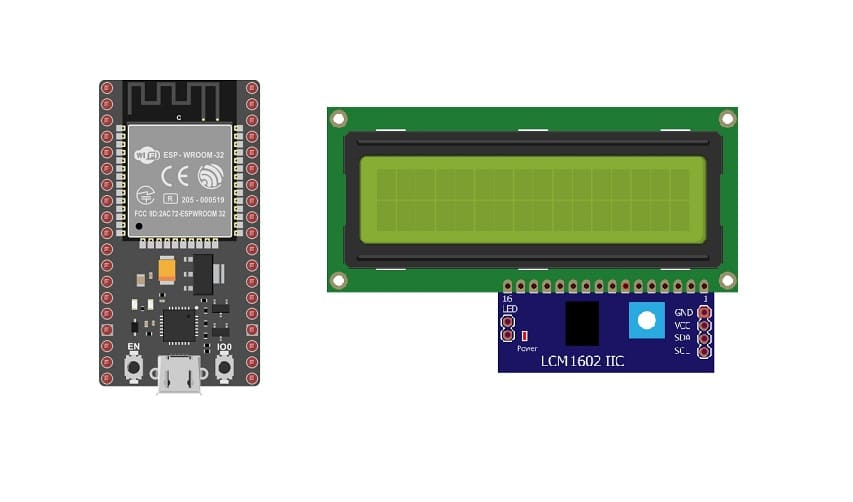
\includegraphics[width=\textwidth]{images/esp32-lcd-i2c-single.jpg}
        \caption{LCD 16x2}
    \end{subfigure}
    \hfill
    \begin{subfigure}[b]{0.19\textwidth}
        \centering
        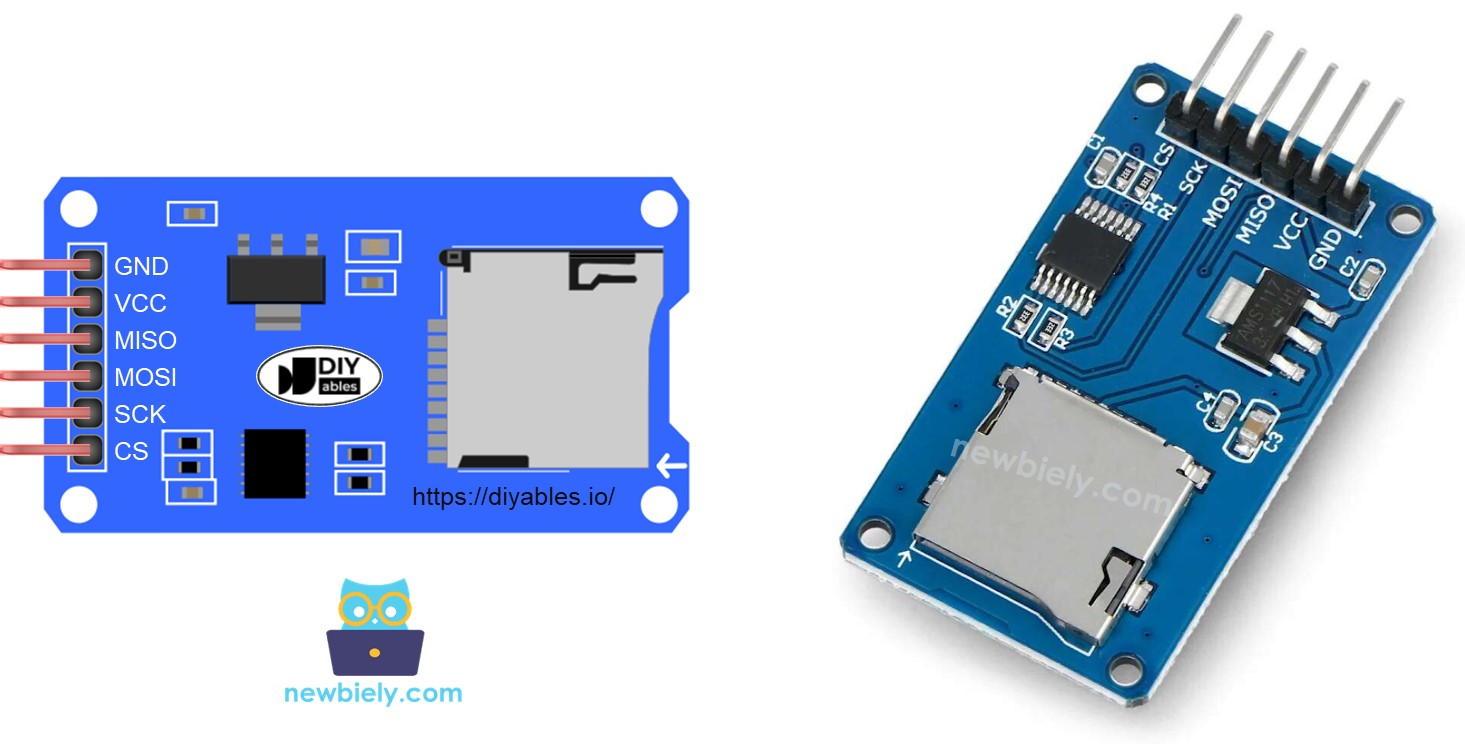
\includegraphics[width=\textwidth]{images/micro-sd-card-module-pinout.jpg}
        \caption{Lecteur SD}
    \end{subfigure}
    \hfill
    \begin{subfigure}[b]{0.19\textwidth}
        \centering
        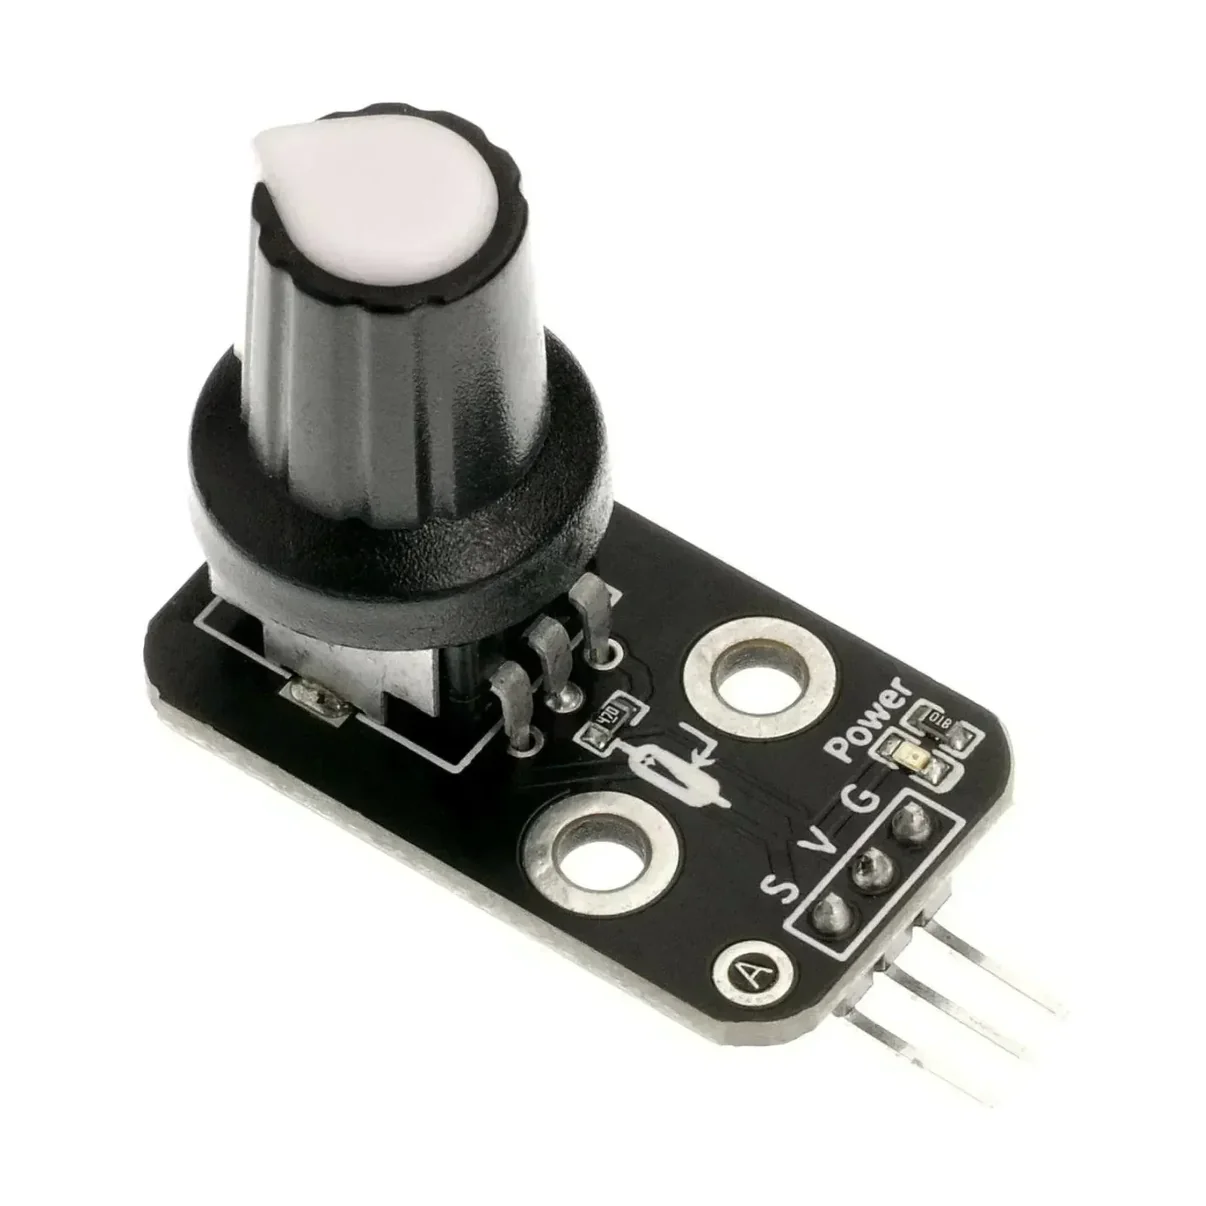
\includegraphics[width=\textwidth]{images/potentiometre_rotatif.png}
        \caption{Potentiomètre}
    \end{subfigure}
    \hfill
    \begin{subfigure}[b]{0.19\textwidth}
        \centering
        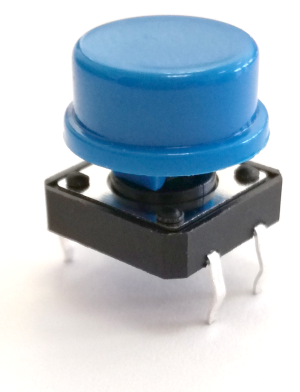
\includegraphics[width=\textwidth]{images/bouton_bleu.png}
        \caption{Boutons}
    \end{subfigure}
    \hfill
    \begin{subfigure}[b]{0.19\textwidth}
        \centering
        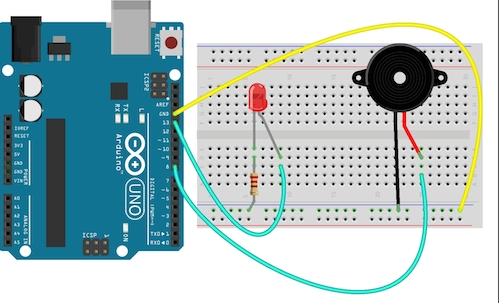
\includegraphics[width=\textwidth]{images/buzzer + led.jpg}
        \caption{Signalisation}
    \end{subfigure}
    \caption{Interfaces locales et modules de traçabilité}
    \label{fig:ihm_systeme}
\end{figure}
\FloatBarrier

Le \textbf{lecteur MicroSD} (interface SPI, format FAT32) joue un rôle critique pour la traçabilité : en l'absence de réseau WiFi, toutes les métriques de traitement sont sauvegardées localement et retransmises automatiquement au broker MQTT dès la reconnexion — mécanisme dit de \textit{Store-and-Forward}.

% -------------------------------------------------------
\section{Sous-système énergétique : autonomie solaire}
% -------------------------------------------------------
Pour garantir un fonctionnement ininterrompu en milieu rural hors réseau, le système \textbf{SMART-SOJA} repose sur une alimentation photovoltaïque dimensionnée selon les principes de calcul de capacité batterie pour systèmes isolés \cite{labouret2017}. Le bilan de puissance des actionneurs est détaillé dans le Tableau \ref{tab:specs_energie} et le synoptique complet de la chaîne de puissance est présenté en \textbf{Annexe \ref{annexe:schema_alim}}.

\begin{table}[H]
    \caption{Bilan énergétique et spécifications d'alimentation}
    \label{tab:specs_energie}
    \centering
    \small
    \renewcommand{\arraystretch}{1.5}
    \rowcolors{2}{white}{lightGray}
    \begin{tabularx}{\textwidth}{|L|L|}
        \hline
        \rowcolor{lightGray}
        \textbf{Paramètre Énergétique} & \textbf{Valeur / Spécification} \\ \hline
        Production (Panneau) & Monocristallin 50~W (Peak) \\ \hline
        Stockage (Batterie) & Plomb-acide 12~V 20~Ah (240~Wh) \\ \hline
        Bilan de puissance crête & 37,85~W (Toutes charges ON) \\ \hline
        Consommation journalière est. & environ 113,5~Wh (pour 3h de travail) \\ \hline
        Autonomie théorique (sans soleil) & environ 1 jour (à 50\% de décharge) \\ \hline
        Conversion & Régulateurs Buck LM2596 (Efficacité > 85\%) \\ \hline
    \end{tabularx}
\end{table}

\textbf{Dimensionnement du système :} Pour valider les choix technologiques du kit de l'entreprise \textbf{QOTTO} (Batterie de 20~Ah et panneau de 50~W), nous avons procédé à un dimensionnement basé sur le besoin réel du prototype.

\begin{enumerate}
    \item \textbf{Étape 1 — Bilan de puissance crête :} La puissance totale est la somme des consommations réelles des composants du prototype (incluant deux résistances et deux ventilateurs pour le séchage) :
    \[ P_{tot} = \underbrace{9,0\text{W}}_{\text{2 Moteurs}} + \underbrace{\mathbf{24,0\text{W}}}_{\text{2 Résistances}} + \underbrace{\mathbf{3,6\text{W}}}_{\text{2 Ventilos}} + \underbrace{1,25\text{W}}_{\text{ESP32}} = \mathbf{37,85~\text{W}} \]
    
    \item \textbf{Étape 2 — Énergie consommée par jour ($E_j$) :} En considérant une utilisation du prototype pendant \textbf{3 heures par jour} (soit environ 18 cycles de traitement), l'énergie totale consommée est :
    \[ E_{jour} = 37,85~\text{W} \times 3~\text{h} \approx \mathbf{113,5~\text{Wh/jour}} \]
    
    \item \textbf{Étape 3 — Validation de la batterie :} La batterie de 12~V et 20~Ah possède une capacité totale de \textbf{240~Wh}. En limitant la décharge à 50~\% pour prolonger sa durée de vie (standard pour les batteries au plomb), l'énergie réellement disponible est de \textbf{120~Wh}.
    \begin{itemize}
        \item \textbf{Conclusion :} 120~Wh (disponibles) $>$ 113,5~Wh (besoin), la batterie est donc bien dimensionnée pour couvrir une session de travail quotidienne en autonomie.
    \end{itemize}

    \item \textbf{Étape 4 — Validation du panneau solaire :} Avec un ensoleillement moyen de 5 heures par jour au Bénin, le panneau de 50~W produit :
    \[ E_{produite} = 50~\text{W} \times 5~\text{h} = \mathbf{250~\text{Wh/jour}} \]
    \begin{itemize}
        \item \textbf{Conclusion :} 250~Wh (produits) $>$ 113,5~Wh (besoin), le panneau recharge la batterie très facilement, offrant une marge de sécurité confortable pour compenser les jours de faible ensoleillement.
    \end{itemize}
\end{enumerate}

% -------------------------------------------------------
\section{Sous-système mécanique : architecture modulaire}
% -------------------------------------------------------
La conception mécanique repose sur une structure modulaire composée d'un châssis porteur accueillant quatre blocs fonctionnels amovibles. Les matériaux ont été sélectionnés selon un compromis robustesse/coût de prototypage (Tableau \ref{tab:specs_mecanique}). Des photographies des matériaux bruts utilisés sont consultables en \textbf{Annexe \ref{annexe:materiaux_mecaniques}}.

\begin{table}[H]
    \caption{Spécifications mécaniques, contraintes et justification des matériaux}
    \label{tab:specs_mecanique}
    \centering
    \small
    \renewcommand{\arraystretch}{1.5}
    \rowcolors{2}{white}{lightGray}
    \begin{tabularx}{\textwidth}{|L|C|L|L|}
        \hline
        \rowcolor{lightGray}
        \textbf{Élément} & \textbf{Masse (kg)} & \textbf{Contrainte / Rigidité} & \textbf{Justification Matériau} \\ \hline
        Châssis porteur & 12,0 & Compression / Haute & Acier (Tubes 40~mm) : Robustesse et soudabilité \\ \hline
        Support Tamis & 0,293 & Vibration / Haute & Inox 304 : Résistance à la corrosion et hygiène \\ \hline
        Support Capteur & 0,1 & Flexion / Moyenne & PLA (3D) : Précision et légèreté \\ \hline
        Roulettes (×4) & 2,0 & Chocs / Élastique & Caoutchouc HD : Absorption des vibrations \\ \hline
    \end{tabularx}
\end{table}
\FloatBarrier

Les quatre blocs fonctionnels (alimentation, nettoyage, séchage et pesée) sont conçus pour être retirés individuellement du châssis. Ce système de glissières et connecteurs rapides facilite grandement la maintenance en milieu rural, évitant ainsi le démontage intégral de la machine.



% -------------------------------------------------------
\section{Méthodologie logicielle : contrôle temps réel}
% -------------------------------------------------------

\subsection{Le système multitâche FreeRTOS}
La gestion simultanée de la sécurité, du contrôle et de la communication Internet des objets sur l'ESP32 nécessite un ordonnancement rigoureux des tâches. Nous utilisons \textbf{FreeRTOS} \cite{freeRTOS}, un noyau temps réel miniature qui offre :
\begin{itemize}
    \item \textbf{Déterminisme :} La lecture des capteurs et le pilotage des actionneurs ne sont jamais interrompus par les tâches réseau.
    \item \textbf{Gestion Multi-Core :} Les deux cœurs de l'ESP32 sont répartis selon la criticité des tâches.
    \item \textbf{Hiérarchie des priorités :} Les tâches de sécurité préemptent systématiquement toutes les autres.
\end{itemize}

Cette organisation logicielle est détaillée dans le Tableau \ref{tab:freertos_sched}.

\begin{table}[H]
    \caption{Hiérarchie et configuration de l'ordonnanceur FreeRTOS}
    \label{tab:freertos_sched}
    \centering
    \small
    \renewcommand{\arraystretch}{1.5}
    \rowcolors{2}{white}{lightGray}
    \begin{tabularx}{\textwidth}{|L|C|L|L|}
        \hline
        \rowcolor{lightGray}
        \textbf{Tâche} & \textbf{Priorité} & \textbf{Justification} & \textbf{Risque en cas de latence} \\ \hline
        \textbf{Task\_Safety} & 4 (Max) & Sécurité critique (Arrêt, Surchauffe) & Endommagement du matériel \\ \hline
        \textbf{Task\_Control} & 3 (Haute) & Ordonnancement GRAFCET & Conflits d'états et blocages \\ \hline
        \textbf{Task\_Sensing} & 2 (Moy.) & Acquisition capteurs (Filtrage) & Mesures erronées ou bruitées \\ \hline
        \textbf{Task\_Actuators} & 2 (Moy.) & Pilotage PWM et Servomoteurs & Réactivité saccadée \\ \hline
        \textbf{Task\_LCD} & 1 (Faible) & Interface locale (I2C) & Affichage figé (non critique) \\ \hline
        \textbf{Task\_MQTT} & 1 (Faible) & Communication Internet des objets et SD & Perte de traçabilité \\ \hline
    \end{tabularx}
\end{table}

Le chronogramme de la Figure \ref{fig:freertos_chronogramme} illustre la dynamique de l'ordonnancement préemptif sur l'ESP32.

\begin{figure}[H]
    \centering
    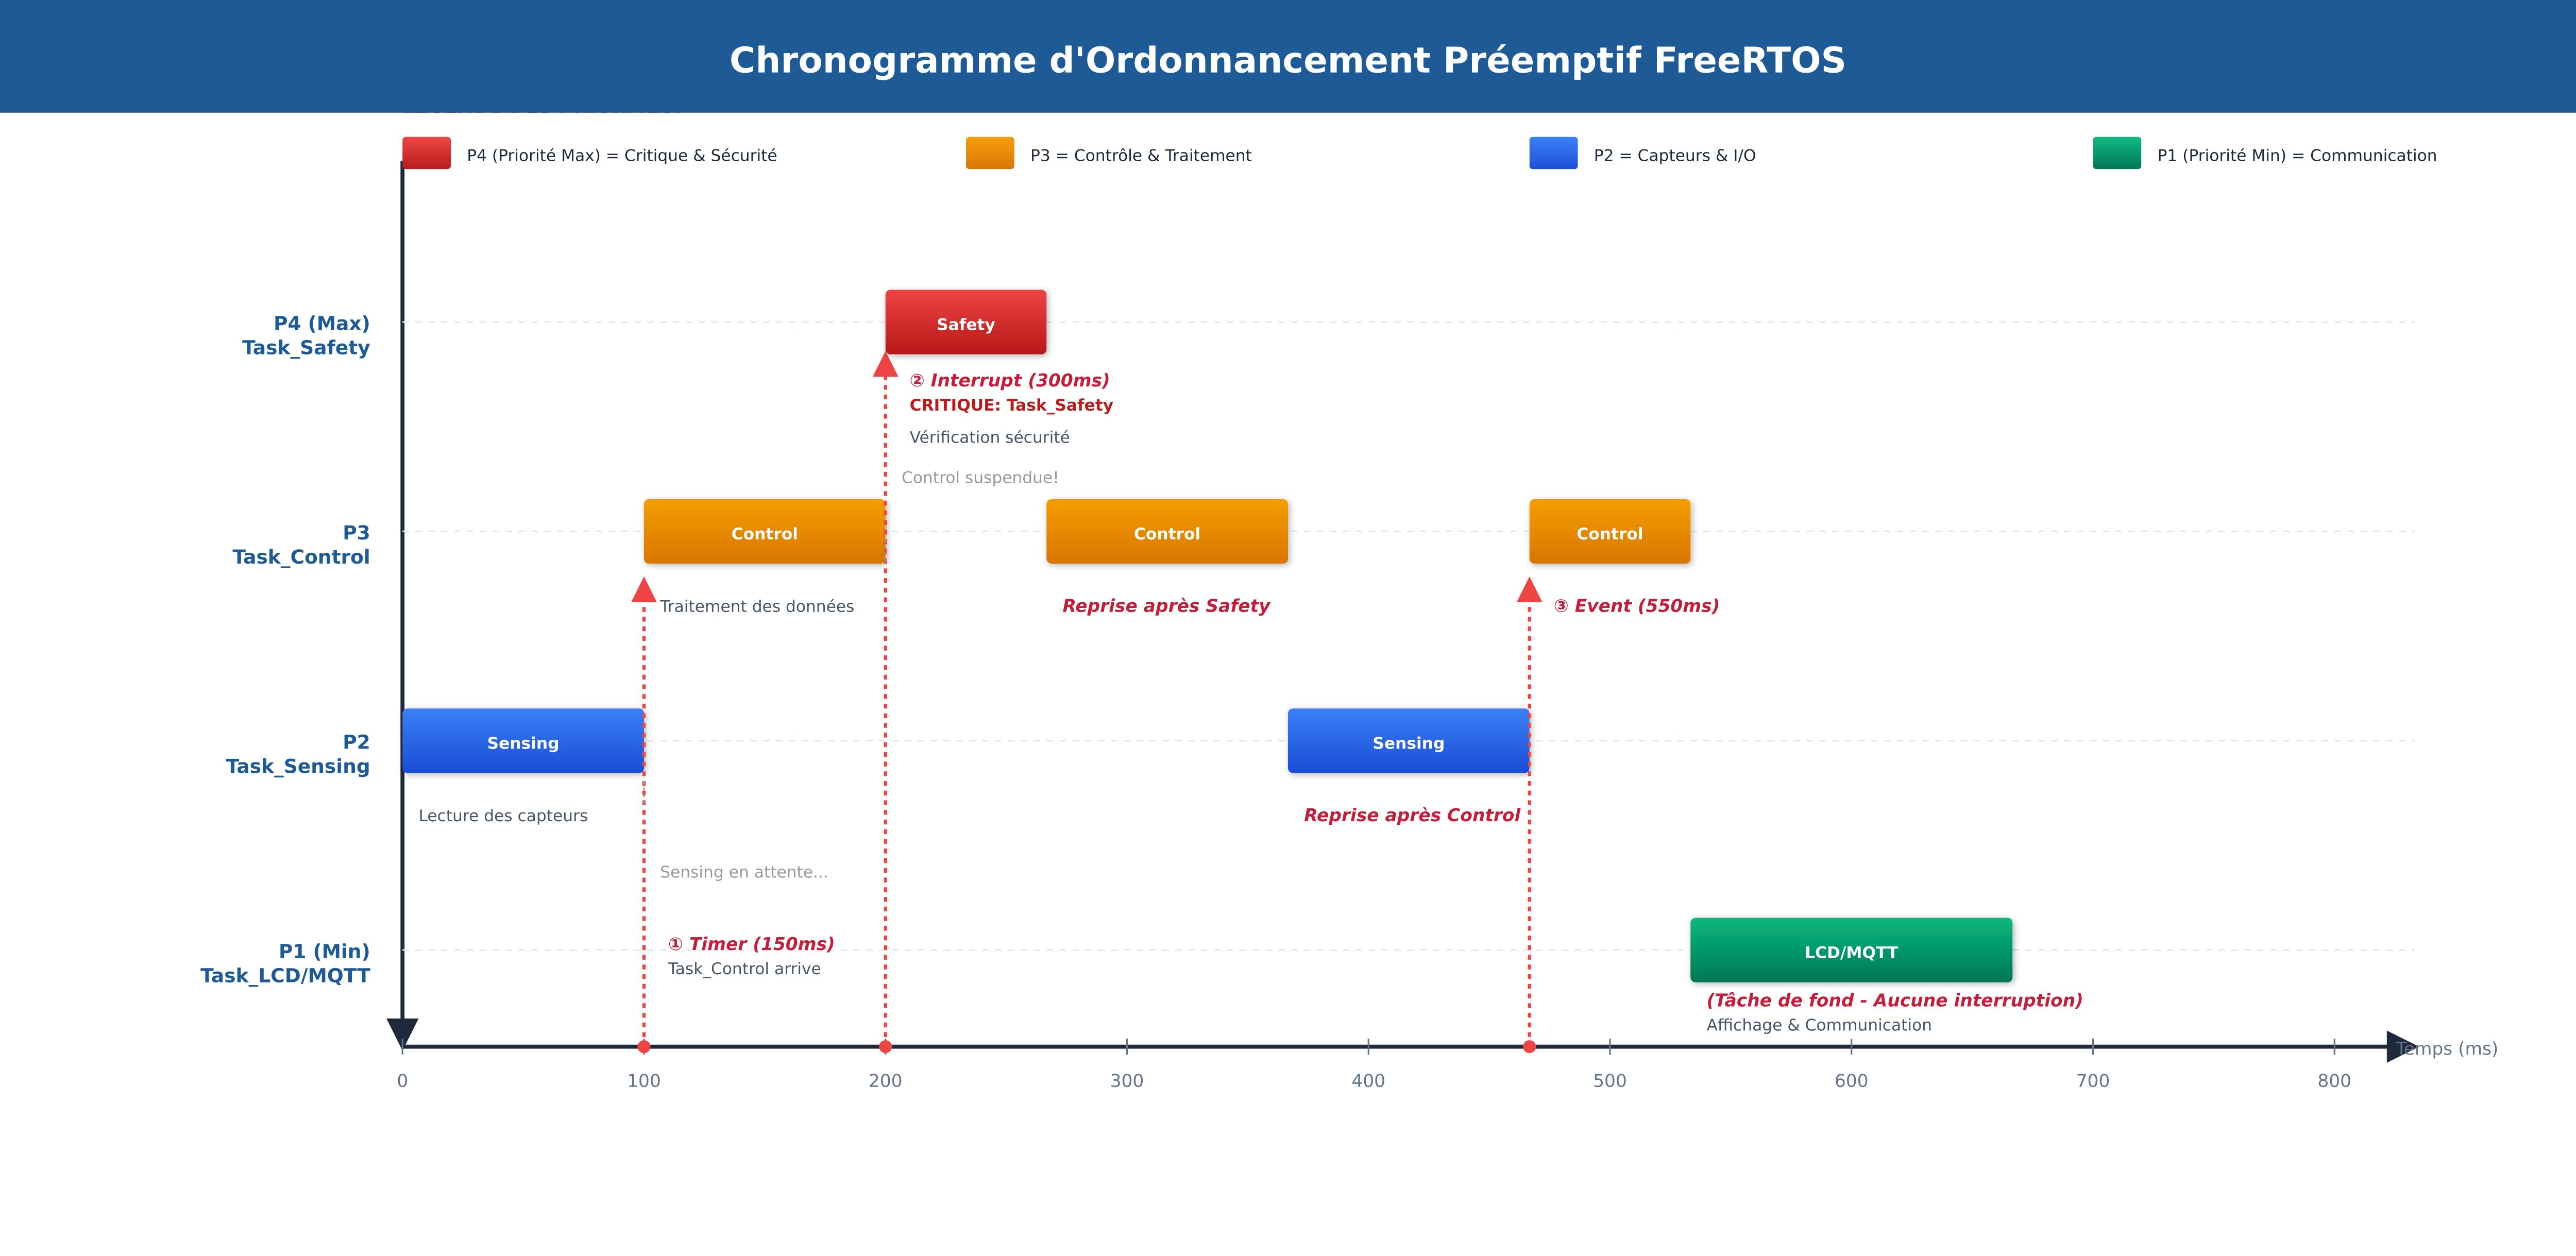
\includegraphics[width=\textwidth]{images/freertos_chronogramme.png}
    \caption{Chronogramme d'ordonnancement préemptif FreeRTOS : Illustration de la préemption et de la hiérarchie des priorités}
    \label{fig:freertos_chronogramme}
\end{figure}

L'ordonnancement repose sur trois principes fondamentaux illustrés par ce graphique :
\begin{enumerate}
    \item \textbf{La Préemption (Interruption) :} Toute tâche de priorité supérieure (ex: \textit{Task\_Safety}) suspend immédiatement l'exécution de la tâche courante (ex: \textit{Task\_Control}), garantissant une réactivité immédiate aux événements critiques.
    \item \textbf{La Reprise Automatique :} Lorsqu'une tâche prioritaire se bloque ou se termine, le noyau FreeRTOS restaure le contexte de la tâche précédemment suspendue, qui reprend exactement là où elle s'était arrêtée.
    \item \textbf{La Gestion des Priorités :} Les tâches de faible priorité (ex: \textit{Task\_LCD / Task\_MQTT}) ne s'exécutent que si aucune tâche plus prioritaire n'est prête à fonctionner, optimisant l'usage du processeur pour les fonctions vitales du système.
\end{enumerate}

\subsection{Modélisation de l'automatisme : le GRAFCET}

La complexité du cycle de traitement du soja — combinant tri mécanique, séchage thermique et pesage électronique — nécessite un outil de modélisation robuste pour garantir une exécution séquentielle sans conflit d'actionneurs. Pour ce faire, nous avons retenu le formalisme du \textbf{GRAFCET} (Graphe Fonctionnel de Commande Étape-Transition), décliné en deux niveaux d'analyse.

\subsubsection{Analyse fonctionnelle (GRAFCET niveau 1)}

Le GRAFCET de niveau 1 décrit le comportement global du système SMART-SOJA du point de vue de l'utilisateur. Le cycle se décompose en trois phases majeures :
\begin{itemize}
    \item \textbf{Phase de préparation :} Le système vérifie la disponibilité de la matière première (Trémie) et la présence d'un réceptacle (Sac) avant d'autoriser l'admission des grains.
    \item \textbf{Phase de traitement :} Elle englobe le nettoyage granulométrique par vibration, suivi d'une analyse critique de l'humidité. Si le soja dépasse le seuil de 12~\%, une séquence de séchage et de brassage est activée de manière itérative jusqu'à conformité.
    \item \textbf{Phase de clôture :} Le lot est transféré vers l'unité de pesée, les données de traçabilité sont enregistrées et le système attend le retrait du sac pour se réinitialiser.
\end{itemize}

\subsubsection{Analyse technologique (GRAFCET niveau 2)}

Le passage au niveau 2 permet de traduire les fonctions précédentes en ordres pilotables par le microcontrôleur ESP32. Cette étape définit les interfaces matérielles :
\begin{itemize}
    \item \textbf{Gestion des entrées :} Utilisation de capteurs infrarouges (IR1 et IR2) pour la détection de présence, et de sondes capacitives reliées aux convertisseurs analogique-numérique (ADC) pour l'humidité.
    \item \textbf{Pilotage des sorties :} Commande de servomoteurs par signaux PWM pour la gestion des vannes, et activation de MOSFETs de puissance pour les éléments thermiques et vibratoires.
\end{itemize}

\subsubsection{Évolutions et logique de cycle}

Pour optimiser le rendement énergétique et la qualité, l'automatisme intègre des structures algorithmiques avancées :
\begin{enumerate}
    \item \textbf{Saut de Séquence :} Si le soja est détecté comme étant déjà sec lors de l'analyse initiale, le système court-circuite l'étape de séchage pour passer directement à l'ensachage, économisant ainsi l'énergie des batteries.
    \item \textbf{Reprise de Séquence (Boucle) :} Un rebouclage est systématiquement effectué après chaque phase de séchage vers l'étape d'analyse, garantissant que seuls les grains conformes à la norme NB 01.07.004 quittent la machine.
    \item \textbf{Sûreté de fonctionnement :} Une évolution parallèle logicielle surveille en permanence le bouton d'arrêt d'urgence et les courants de fuite, capable d'interrompre le cycle à n'importe quelle étape.
\end{enumerate}

\FloatBarrier

\textbf{Double validation de l'humidité :} L'ensachage n'est autorisé que si les deux sondes Soil1 \textit{ET} Soil2 confirment individuellement $H \leq 12~\%$. Cette double validation prévient les hétérogénéités verticales du lot et les défauts de capteur isolé :
\begin{align*}
\text{Sortie\_séchage} &= (S_1 \leq 12~\%) \text{ ET } (S_2 \leq 12~\%) \\
\text{Déclenchement\_séchage} &= (S_1 > 12~\%) \text{ OU } (S_2 > 12~\%)
\end{align*}

L'ensemble de ces règles logiques et technologiques est synthétisé dans le GRAFCET de la Figure \ref{fig:grafcet_systeme}.

\begin{figure}[H]
    \centering
    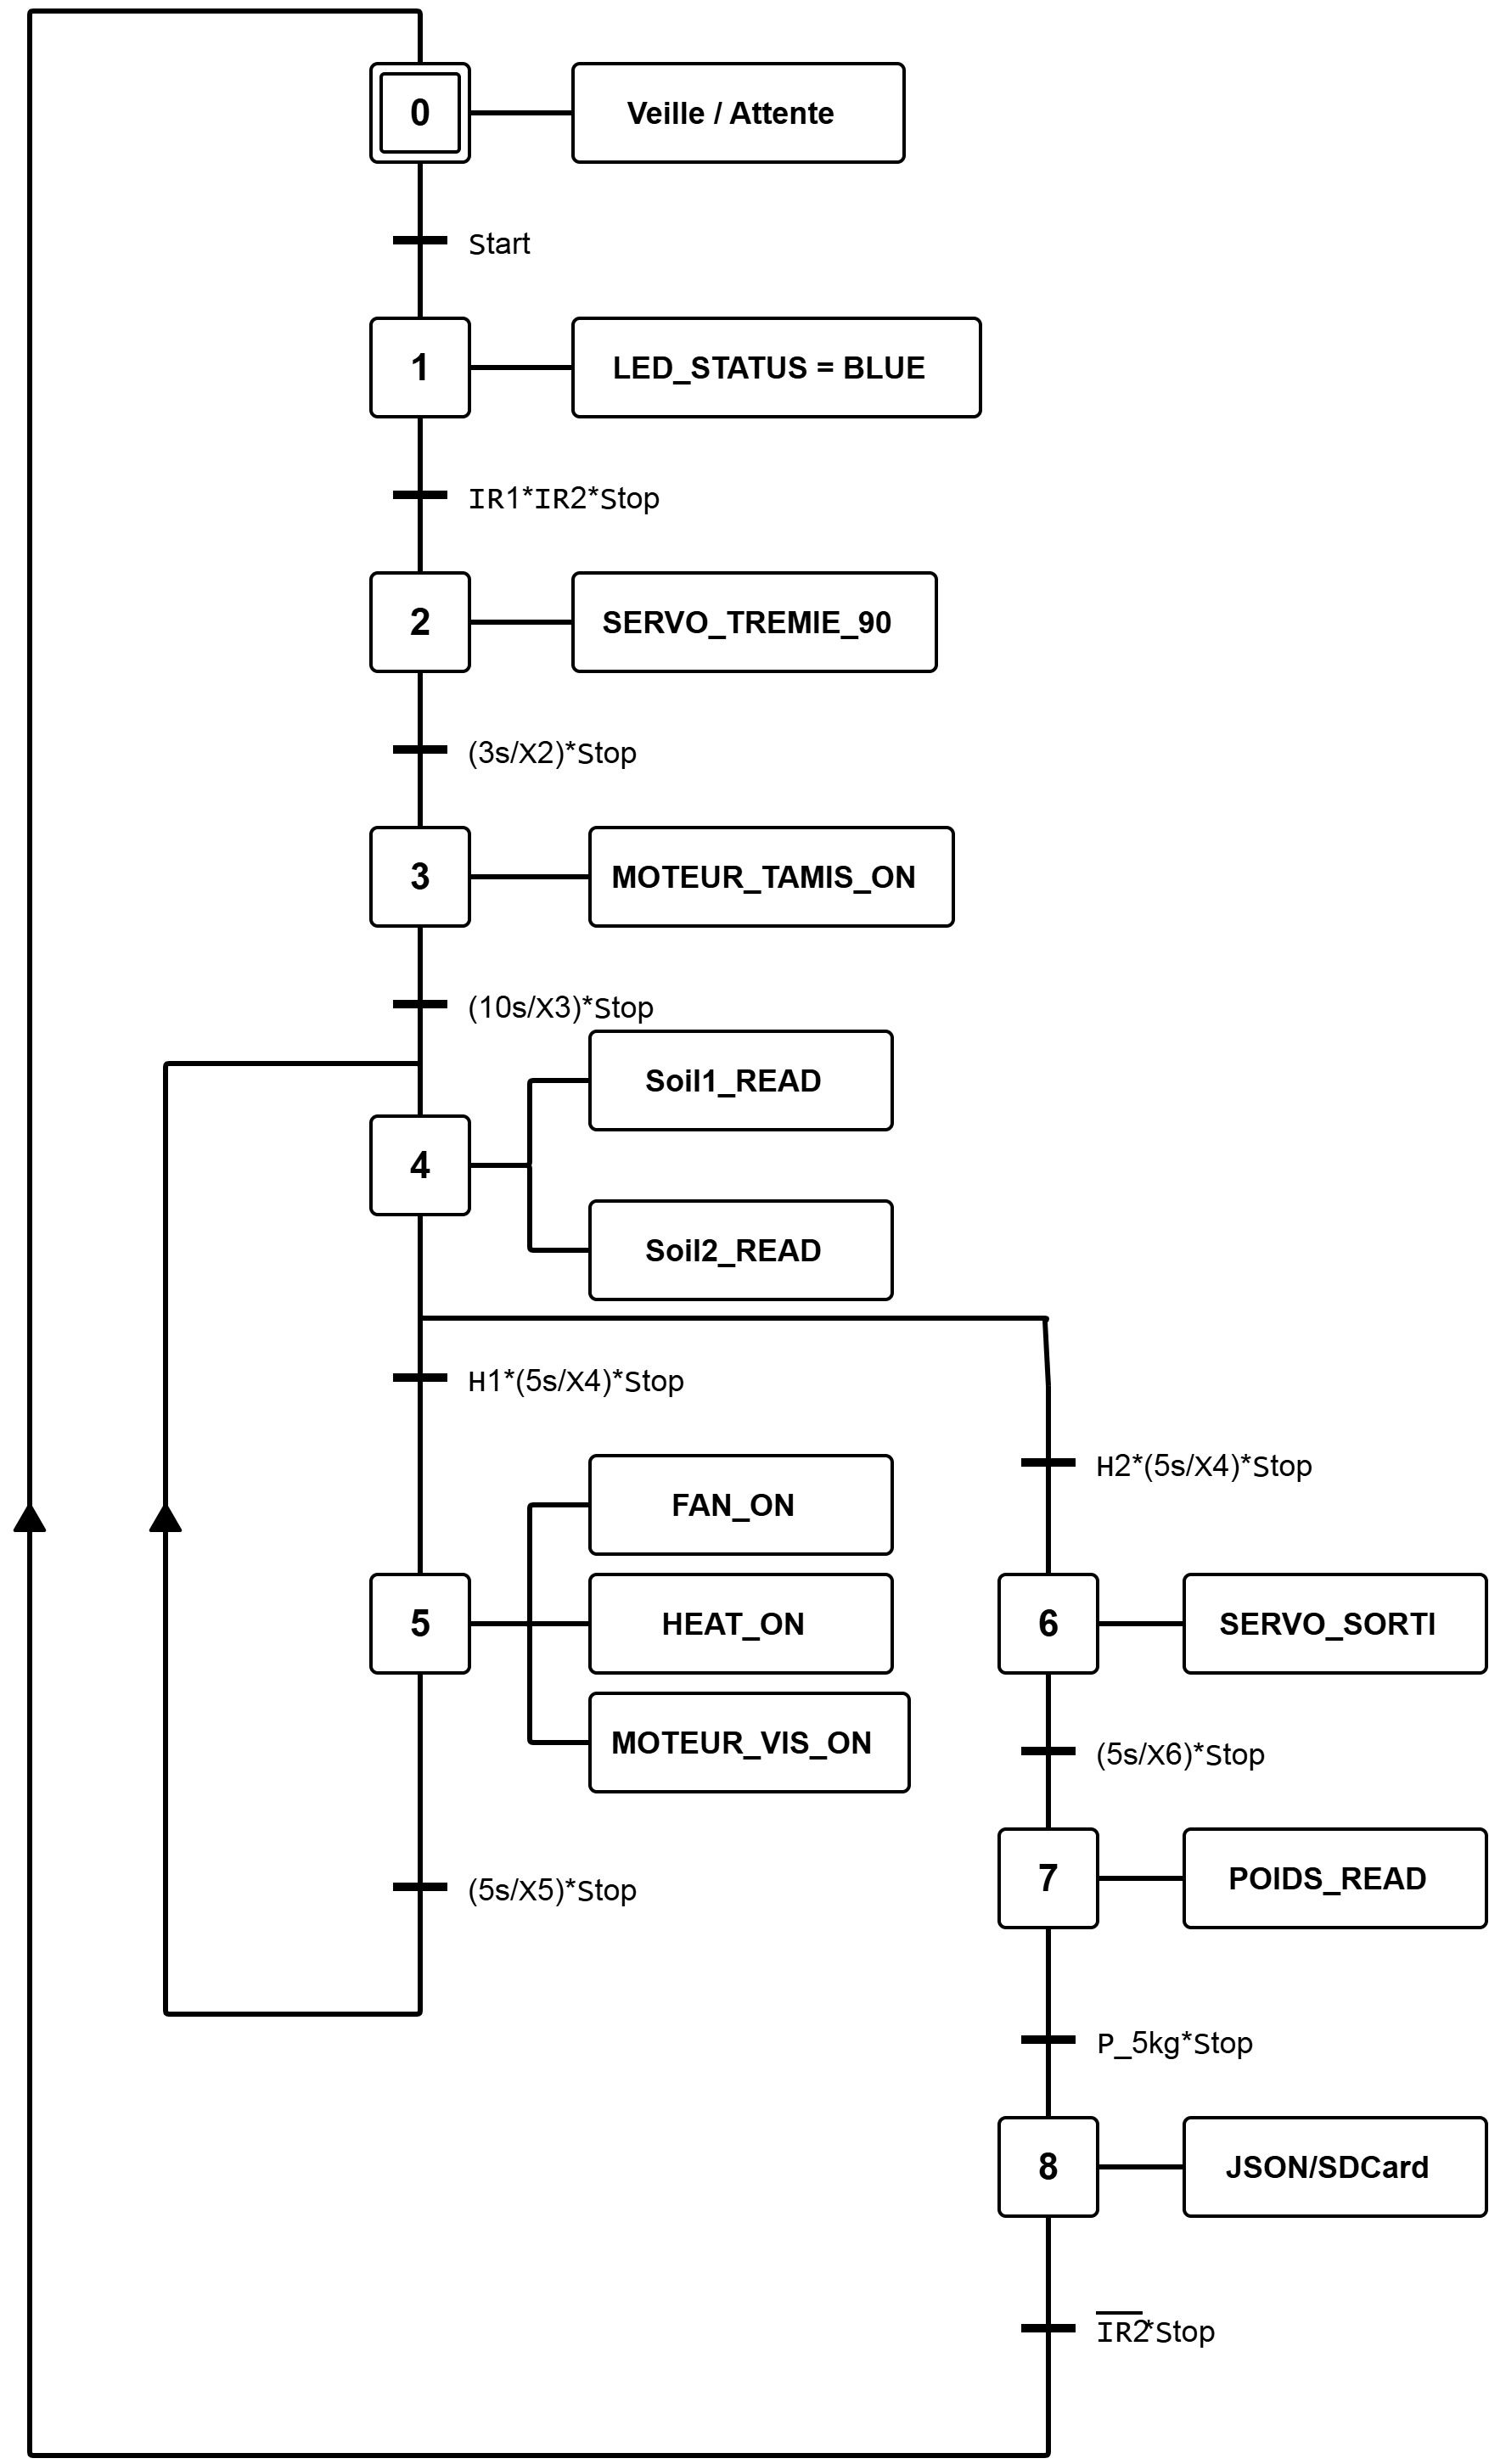
\includegraphics[width=0.6\textwidth]{images/grafcet_smart.png}
    \caption{Algorithme de contrôle séquentiel du système (GRAFCET Niveau 2)}
    \label{fig:grafcet_systeme}
\end{figure}


\subsection{Communication et traçabilité numérique}

Une fois le cycle de traitement validé par le GRAFCET, les données doivent être exportées pour assurer la traçabilité du lot. Le protocole \textbf{MQTT} (architecture Publication/Abonnement) est retenu pour sa légèreté et sa robustesse sur les réseaux à faible bande passante \cite{mqtt_org}. L'utilisation du format \textbf{JSON} garantit quant à elle l'interopérabilité des données entre l'Edge et le Cloud \cite{hanes2017}.

À chaque fin de cycle, la machine génère un \textbf{passeport numérique} au format \textbf{JSON}. Ce message regroupe l'ensemble des métriques de traçabilité (identifiant unique, horodatage, humidité moyenne et poids final) et est publié vers le broker central.

En cas de perte de connexion, ces données sont archivées sur la carte MicroSD et renvoyées dès le rétablissement du signal (\textit{Store-and-Forward}).

% Fin de la section méthodes


% -------------------------------------------------------
% PARTIE 3 : CONCEPTION ET IMPLÉMENTATION
% -------------------------------------------------------

% ---- SECTION CONCEPTION ET IMPLÉMENTATION ----

% -------------------------------------------------------
\section{Environnement de conception et de développement}
Pour mener à bien ce projet mécatronique, plusieurs outils professionnels de conception et de développement ont été mobilisés. Ils permettent de garantir la précision des modèles et l'interopérabilité des données.

\subsection{Conception mécanique et électronique}
\begin{itemize}
    \item \textbf{SolidWorks (Dassault Systèmes) :} Utilisé pour la modélisation 3D intégrale du prototype, les simulations d'assemblage et la génération des mises en plan techniques. C'est le standard industriel pour la conception de systèmes mécaniques complexes.
    \item \textbf{KiCad EDA :} Suite logicielle open-source retenue pour la saisie schématique et le routage du PCB. Sa flexibilité et sa gratuité en font un outil idéal pour le prototypage rapide en milieu académique et professionnel.
\end{itemize}

\subsection{Développement logiciel}
\begin{itemize}
    \item \textbf{Arduino IDE :} Utilisé pour le codage, la compilation et le téléversement du firmware sur l'ESP32. Sa vaste bibliothèque de pilotes facilite l'interfaçage des capteurs et la gestion du WiFi.
    \item \textbf{VS Code (Visual Studio Code) :} Retenu pour le développement du tableau de bord Internet des objets (HTML/JS) en raison de sa gestion avancée du versionnement (Git) et de son écosystème d'extensions.
\end{itemize}

\begin{figure}[H]
    \centering
    % Première ligne : Conception
    \begin{subfigure}[b]{0.45\textwidth}
        \centering
        
\includegraphics[height=3cm]{images/logo_solidwork.png}
        \caption{SolidWorks (CAO)}
    \end{subfigure}
    \hfill
    \begin{subfigure}[b]{0.45\textwidth}
        \centering
        
\includegraphics[height=3cm]{images/logo_kicad.png}
        \caption{KiCad (EDA)}
    \end{subfigure}
    
    \vspace{0.8cm}
    
    % Deuxième ligne : Développement
    \begin{subfigure}[b]{0.45\textwidth}
        \centering
        
\includegraphics[height=3cm]{images/logo_arduino.png}
        \caption{Arduino IDE (Firmware)}
    \end{subfigure}
    \hfill
    \begin{subfigure}[b]{0.45\textwidth}
        \centering
        
\includegraphics[height=3cm]{images/Visual-Studio-Code-logo.png}
        \caption{VS Code (Tableau de bord IoT)}
    \end{subfigure}
    \caption{Écosystème logiciel utilisé pour le projet SMART-SOJA}
    \label{fig:logos_logiciels}
\end{figure}
\FloatBarrier

\section{Conception électronique : le circuit imprimé (PCB)}

Le schéma électronique global, regroupant l'ensemble des blocs fonctionnels, est consultable en \textbf{Annexe \ref{annexe:schema_global}}.

\subsection{Segmentation fonctionnelle de la conception}
Pour garantir une maintenance aisée et minimiser les interférences électromagnétiques (EMI) entre signaux de puissance et de commande, la conception est segmentée en cinq blocs fonctionnels dès la saisie schématique :

\begin{enumerate}
    \item \textbf{Zone Alimentation (Figure \ref{fig:zone_alim}) :} Régulateur Buck \textbf{LM2596} générant un rail 5~V / 2~A depuis la source 12~V. La logique 3,3~V est assurée par le régulateur interne de l'ESP32.
    \begin{figure}[H]
        \centering
        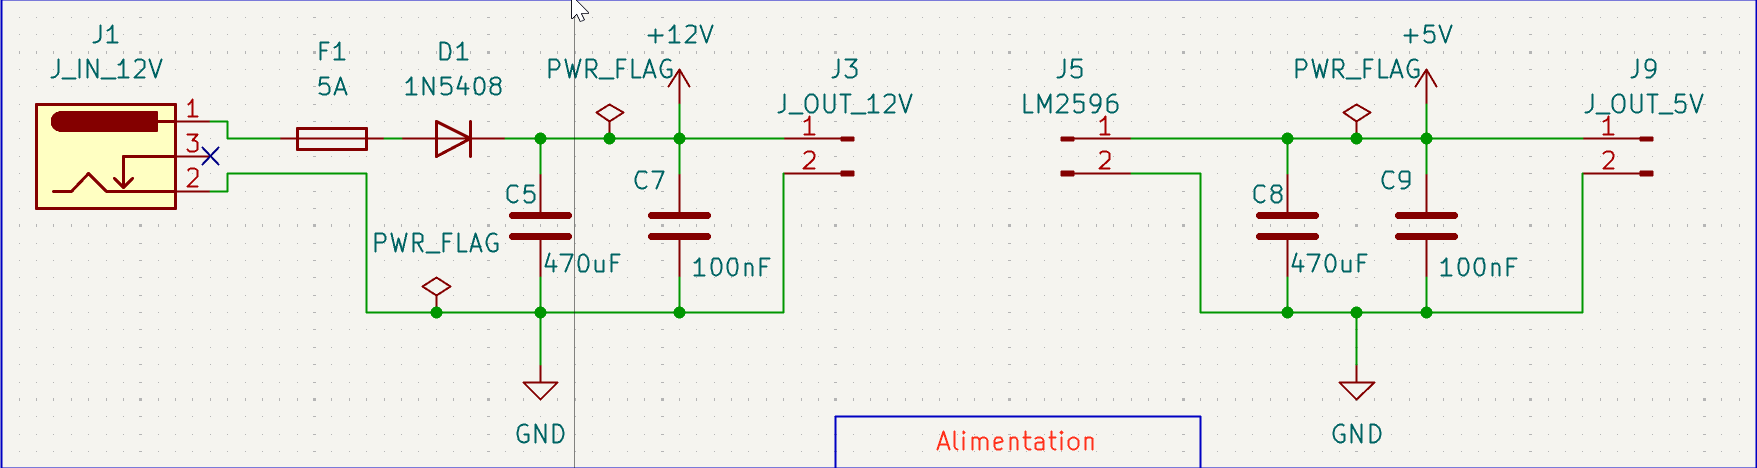
\includegraphics[width=0.55\textwidth]{images/image_circuit_zone-alimentation.PNG}
        \caption{Zone d'alimentation multi-tensions}
        \label{fig:zone_alim}
    \end{figure}

    \item \textbf{Zone ESP32 (Figure \ref{fig:zone_esp32}) :} L'affectation des broches a été optimisée pour éviter les conflits avec les \textit{strapping pins} (GPIO 0, 2, 12, 15) critiques au démarrage.
    \begin{figure}[H]
        \centering
        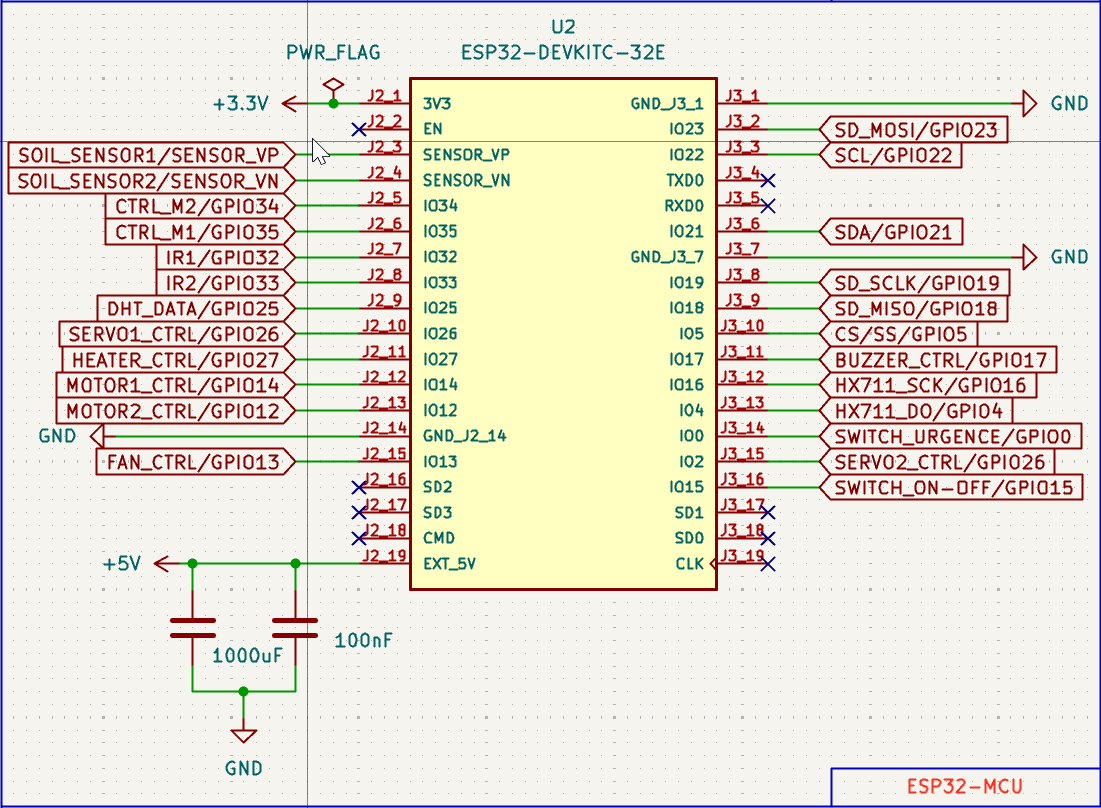
\includegraphics[width=0.55\textwidth]{images/image_circuit_zone-esp32.PNG}
        \caption{Unité de traitement centrale ESP32}
        \label{fig:zone_esp32}
    \end{figure}

    \item \textbf{Zone Puissance (Figure \ref{fig:zone_act}) :} Chaque canal MOSFET IRLZ44N intègre une résistance de grille de 220~$\Omega$, une résistance de rappel pull-down de 10~k$\Omega$ et une diode de roue libre \textbf{1N5408} contre les retours inductifs des moteurs.
    \begin{figure}[H]
        \centering
        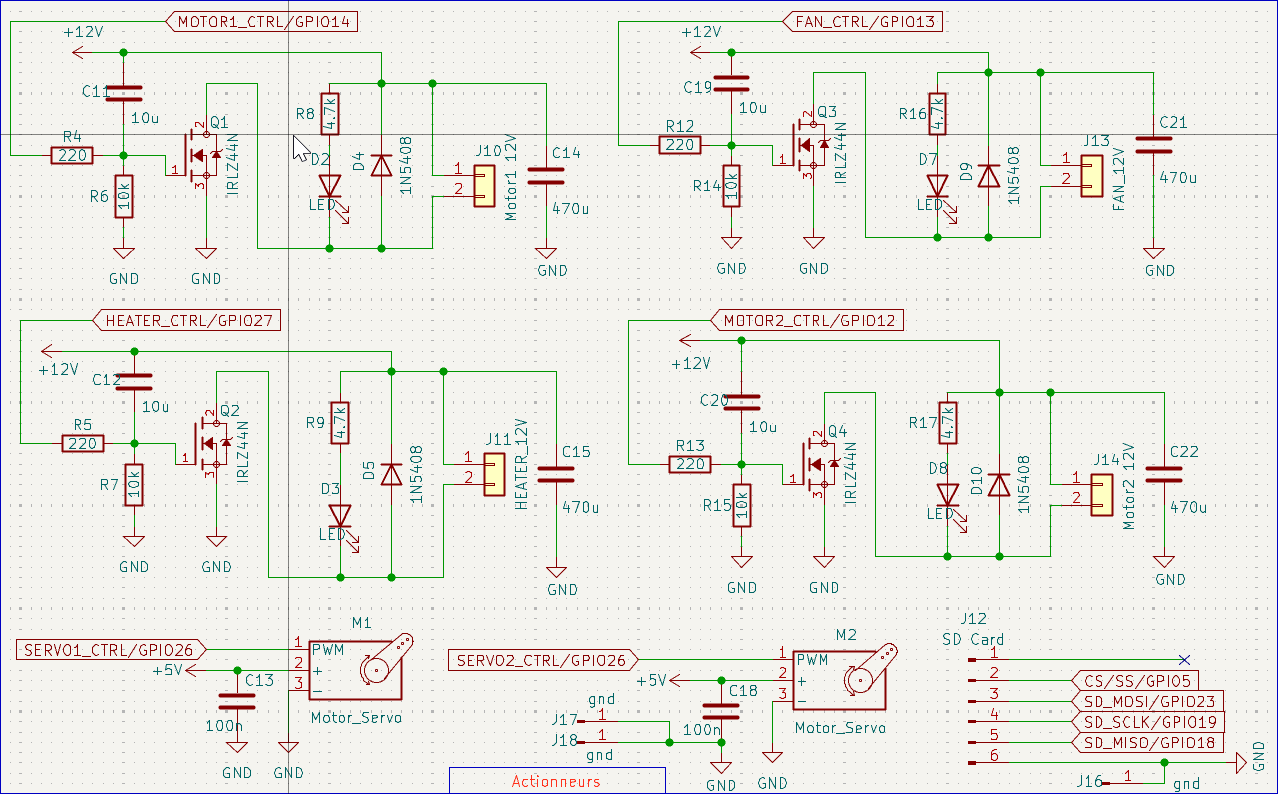
\includegraphics[width=0.55\textwidth]{images/image_circuit_zone-actionneurs.PNG}
        \caption{Étage de puissance avec protections inductives}
        \label{fig:zone_act}
    \end{figure}

    \item \textbf{Zone Acquisition (Figure \ref{fig:zone_cap}) :} Interfaces pour les signaux analogiques (Sondes capacitives sur GPIO 36/39) et numériques (HX711 sur GPIO 25, DHT22, capteurs IR sur GPIO 32/33).
    \begin{figure}[H]
        \centering
        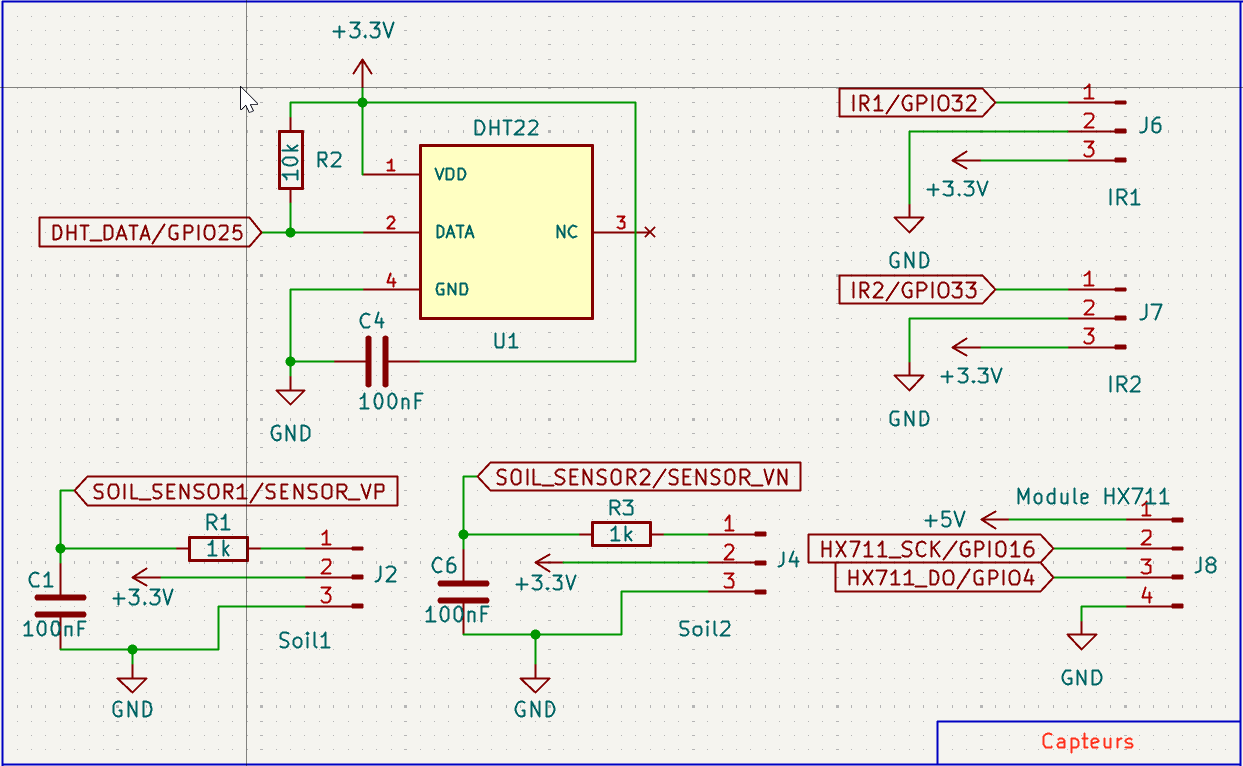
\includegraphics[width=0.55\textwidth]{images/image_circuit_zone-capteurs.PNG}
        \caption{Interface d'acquisition des capteurs}
        \label{fig:zone_cap}
    \end{figure}

    \item \textbf{Zone IHM (Figure \ref{fig:zone_ihm}) :} Gestion du bus I2C (LCD), du bus SPI (carte SD) et des signaux PWM (buzzer, servomoteur, boutons).
    \begin{figure}[H]
        \centering
        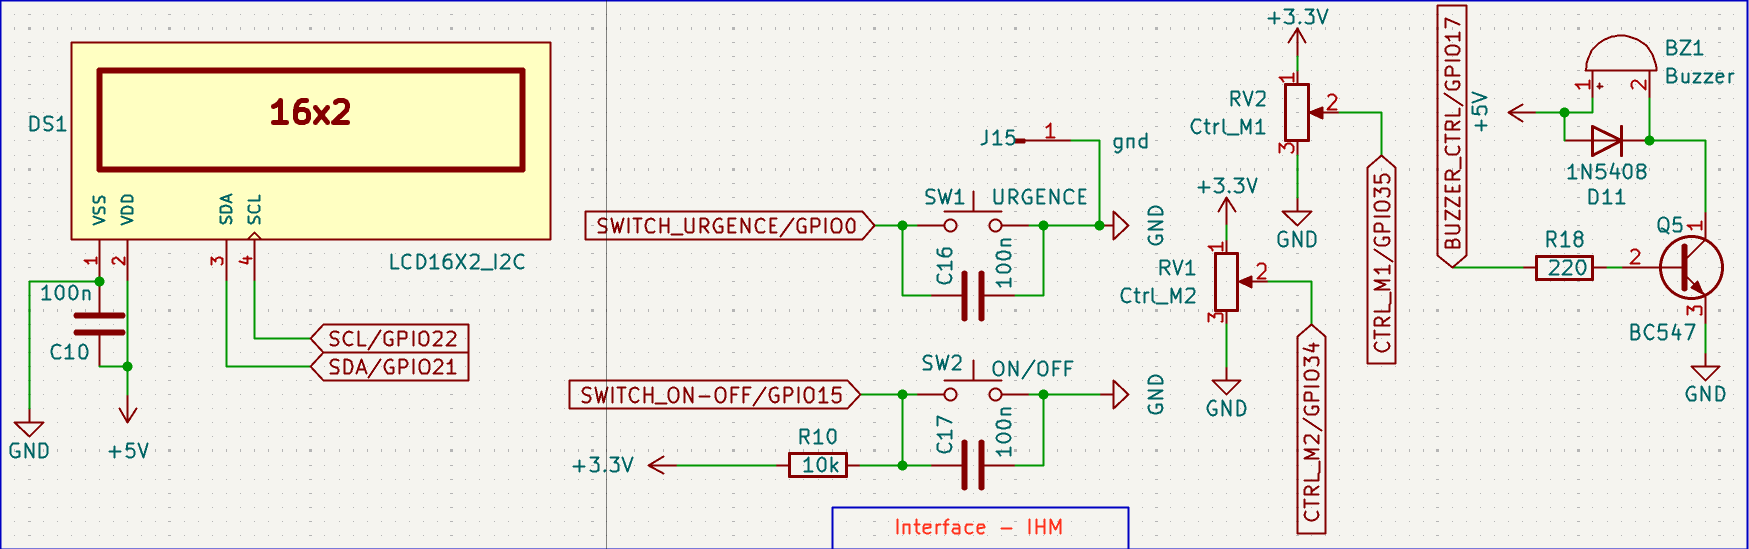
\includegraphics[width=0.55\textwidth]{images/image_circuit_zone-ihm.PNG}
        \caption{Interface Homme-Machine locale}
        \label{fig:zone_ihm}
    \end{figure}
\end{enumerate}
\FloatBarrier

Le routage sous KiCad a été réalisé sur une \textbf{seule couche (Bottom Layer)} pour simplifier la fabrication du prototype. Les pistes de puissance sont dimensionnées à une largeur minimale de \textbf{1~mm} pour supporter les charges inductives sans échauffement. Un plan de masse (Ground Pour) a été généré sur cette face unique pour assurer l'intégrité du signal et limiter les boucles de masse.

La modélisation 3D du PCB a permis de valider l'absence de collision mécanique entre composants volumineux avant fabrication. Les vues détaillées (routage, faces 3D) sont consultables en \textbf{Annexe \ref{annexe:routage_pcb}} et \textbf{Annexe \ref{annexe:vues_3d_pcb}}.

% -------------------------------------------------------
\section{Conception mécanique : architecture modulaire}
% -------------------------------------------------------
La conception mécanique a été réalisée sous \textbf{SolidWorks} selon une architecture modulaire en quatre blocs fonctionnels indépendants (Figure \ref{fig:cad_4blocs}), montés sur un châssis porteur mobile.

\begin{figure}[H]
    \centering
    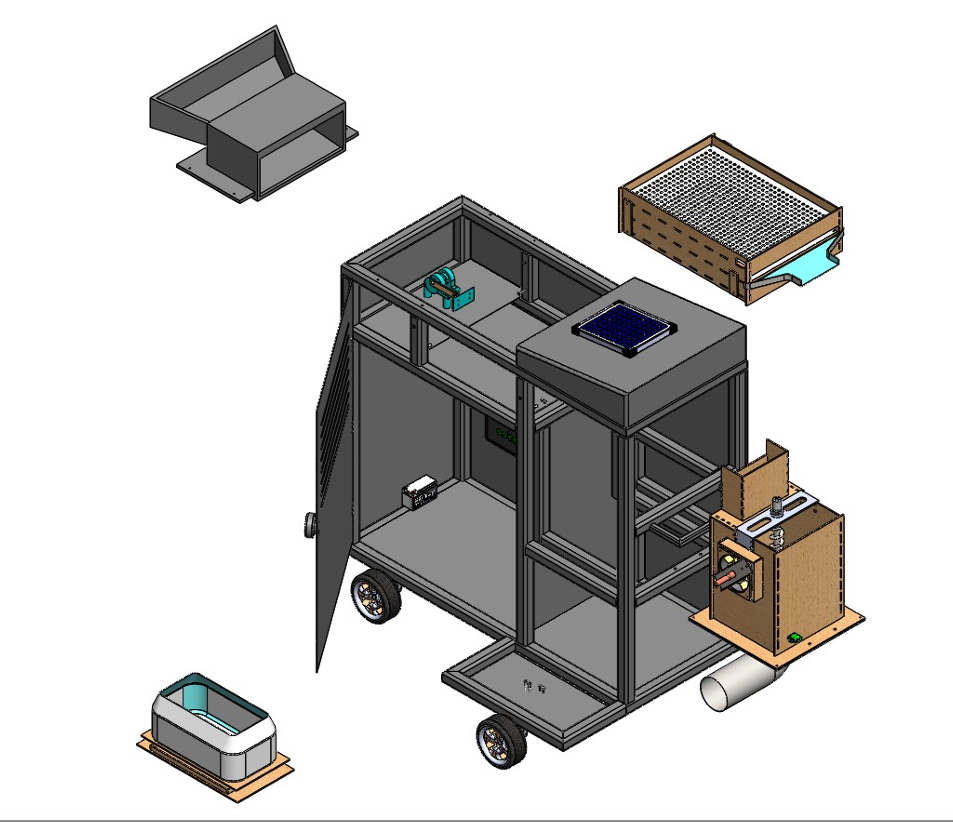
\includegraphics[width=0.85\textwidth]{images/Vue_modulaire_3D.PNG}
    \caption{Architecture modulaire du système SMART-SOJA — Vue d'ensemble CAO}
    \label{fig:cad_4blocs}
\end{figure}
\FloatBarrier


\begin{enumerate}
    \item \textbf{Bloc 1 — Unité d'entrée (Trémie) :} Trémie pyramidale à écoulement gravitaire, pilotée par le servomoteur SG90. Le capteur IR1 confirme la présence de soja avant l'ouverture.

    \item \textbf{Bloc 2 — Unité de nettoyage et vibration :} Deux tamis inox superposés montés sur suspensions élastiques. Le moteur JGA25-370 génère les oscillations via un système poulie-tige de transmission, assurant la séparation granulométrique.

    \item \textbf{Bloc 3 — Unité de séchage et analyse (Figure \ref{fig:sechage_pesee_cad}) :}
    \begin{itemize}
        \item \textbf{Vis sans fin} (type Archimède) : brassage mécanique continu pour un séchage homogène.
        \item \textbf{Ensemble Ventilateur + Résistance Chauffante} : circulation d'air chaud.
        \item \textbf{Boîtiers capteurs} : logements dédiés aux deux sondes capacitives (Soil1/Soil2) et au DHT22.
    \end{itemize}

    \begin{figure}[H]
        \centering
        \begin{subfigure}[b]{0.48\textwidth}
            \centering
            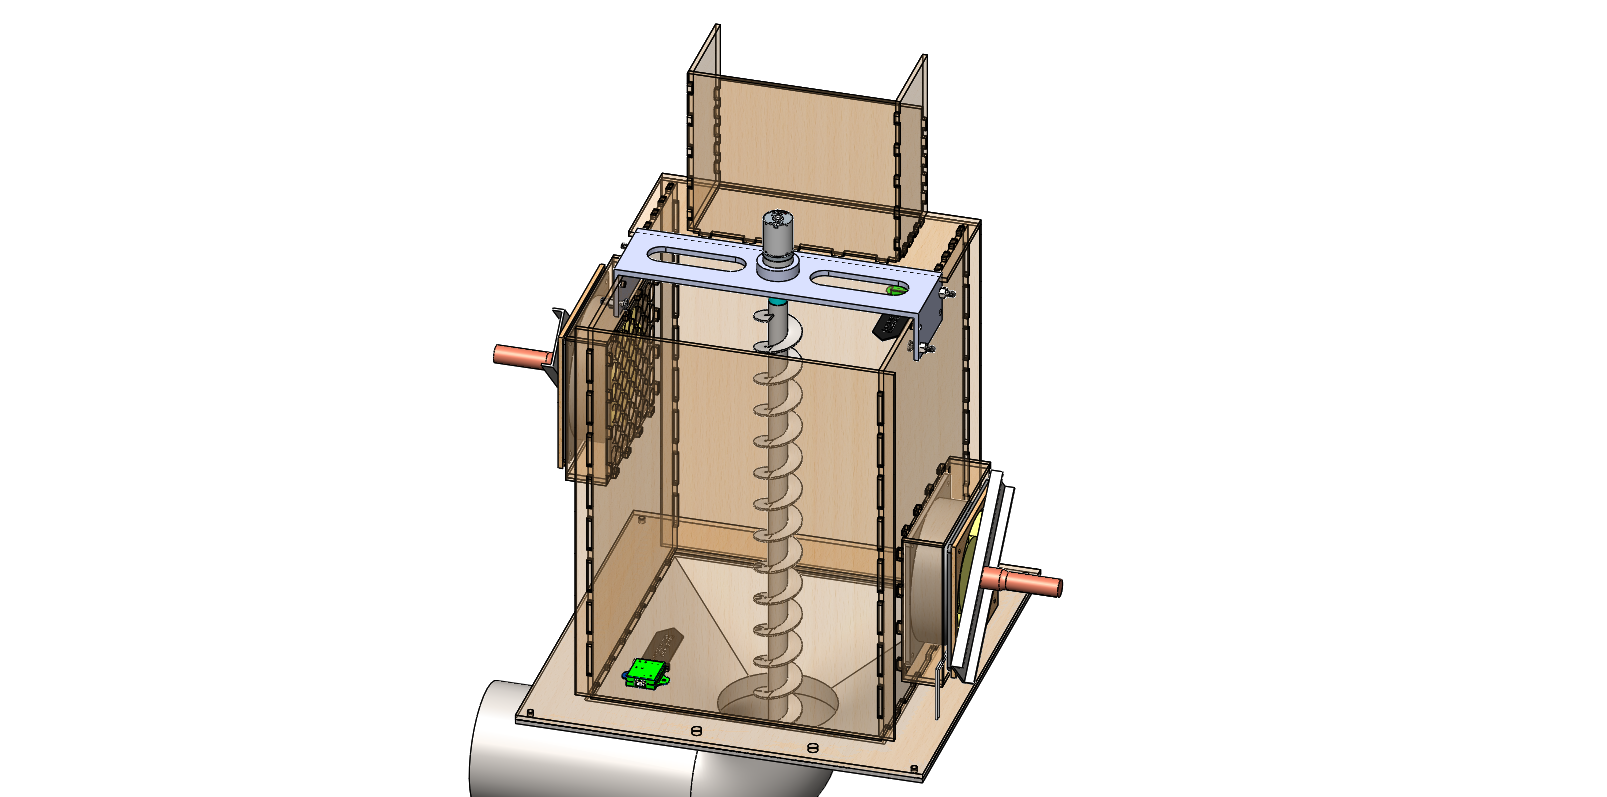
\includegraphics[width=\textwidth]{images/systeme_sechage.PNG}
            \caption{Unité de séchage (Vue 3D)}
        \end{subfigure}
        \hfill
        \begin{subfigure}[b]{0.48\textwidth}
            \centering
            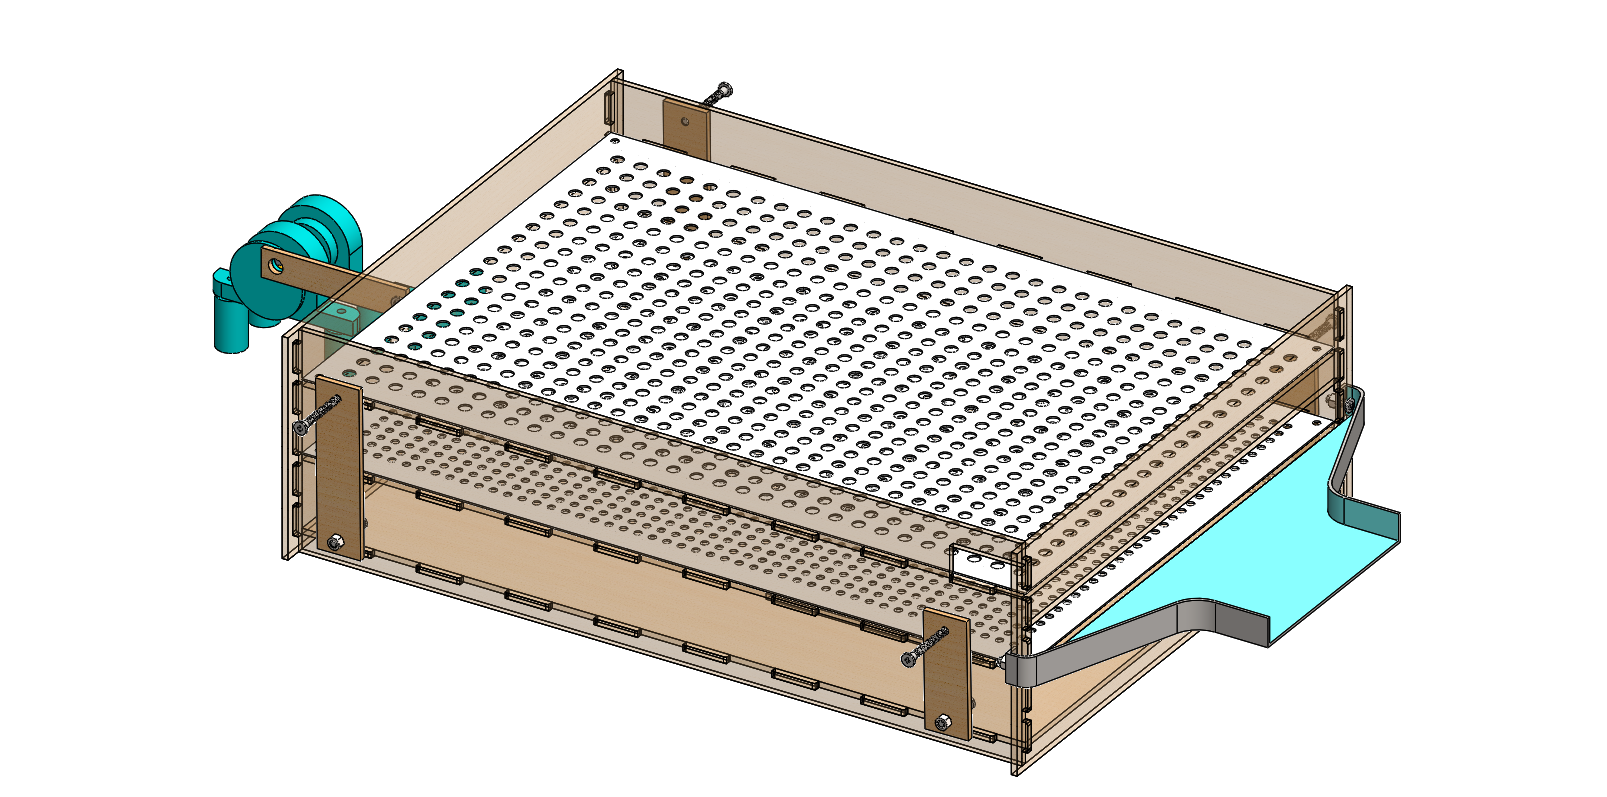
\includegraphics[width=\textwidth]{images/systeme_tami.PNG}
            \caption{Unité de tamisage (Vue 3D)}
        \end{subfigure}
        \caption{Détails des blocs de traitement mécanique sous SolidWorks}
        \label{fig:sechage_pesee_cad}
    \end{figure}
    \FloatBarrier


    \item \textbf{Bloc 4 — Unité de pesée et réception :} Support cellule de charge (Load Cell HX711) avec plateau de réception finale. Le capteur IR2 confirme le retrait du sac en fin de cycle.
\end{enumerate}

\begin{figure}[H]
    \centering
    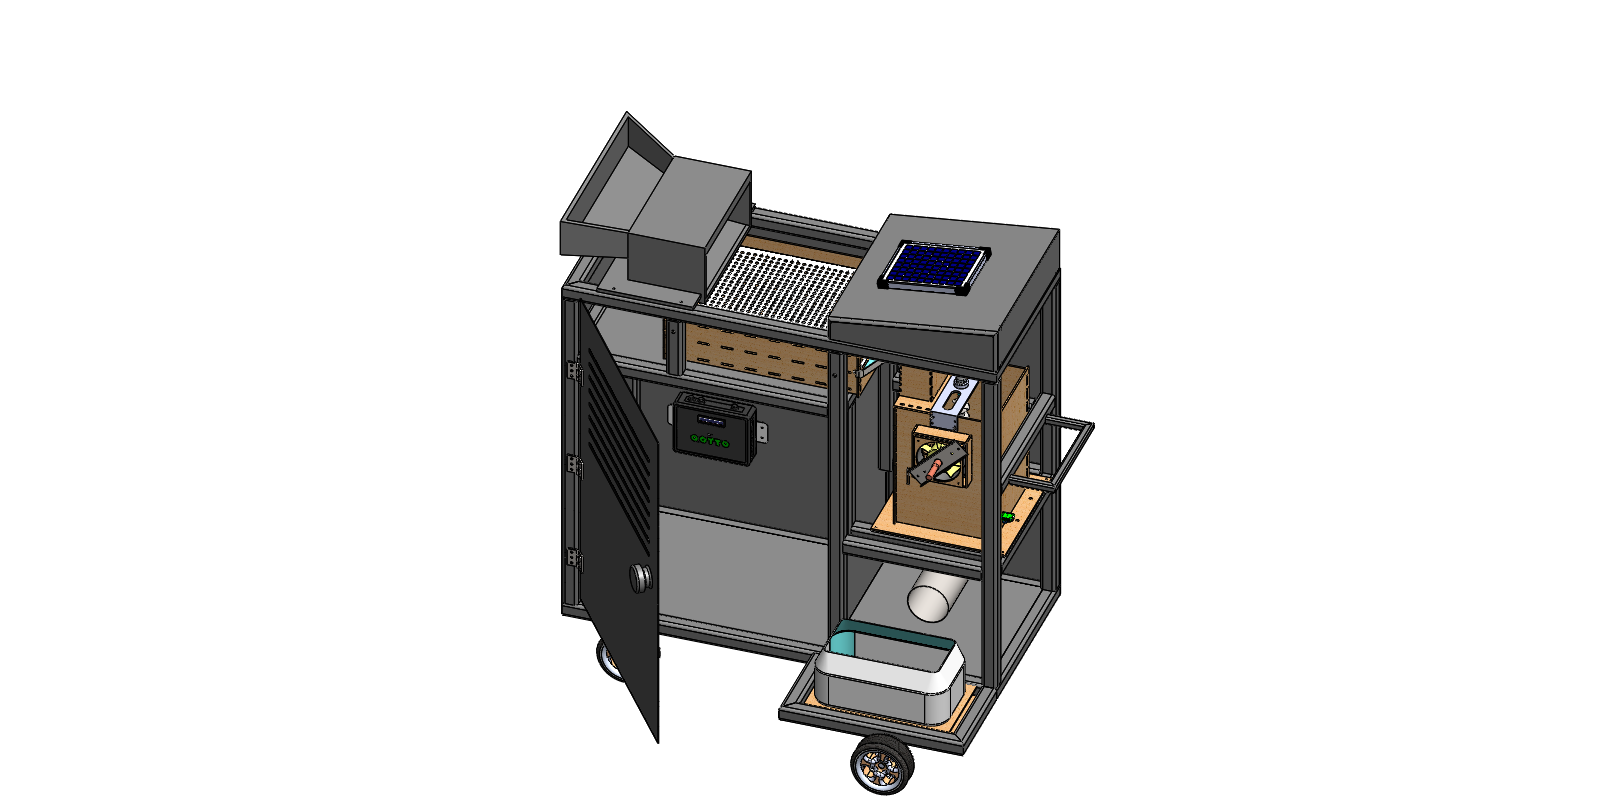
\includegraphics[width=1.02\textwidth]{images/Smart-Soja.PNG}
    \caption{Vue d'ensemble du prototype SMART-SOJA assemblé (SolidWorks)}
    \label{fig:systeme_complet}
\end{figure}
\FloatBarrier

\begin{figure}[H]
    \centering
    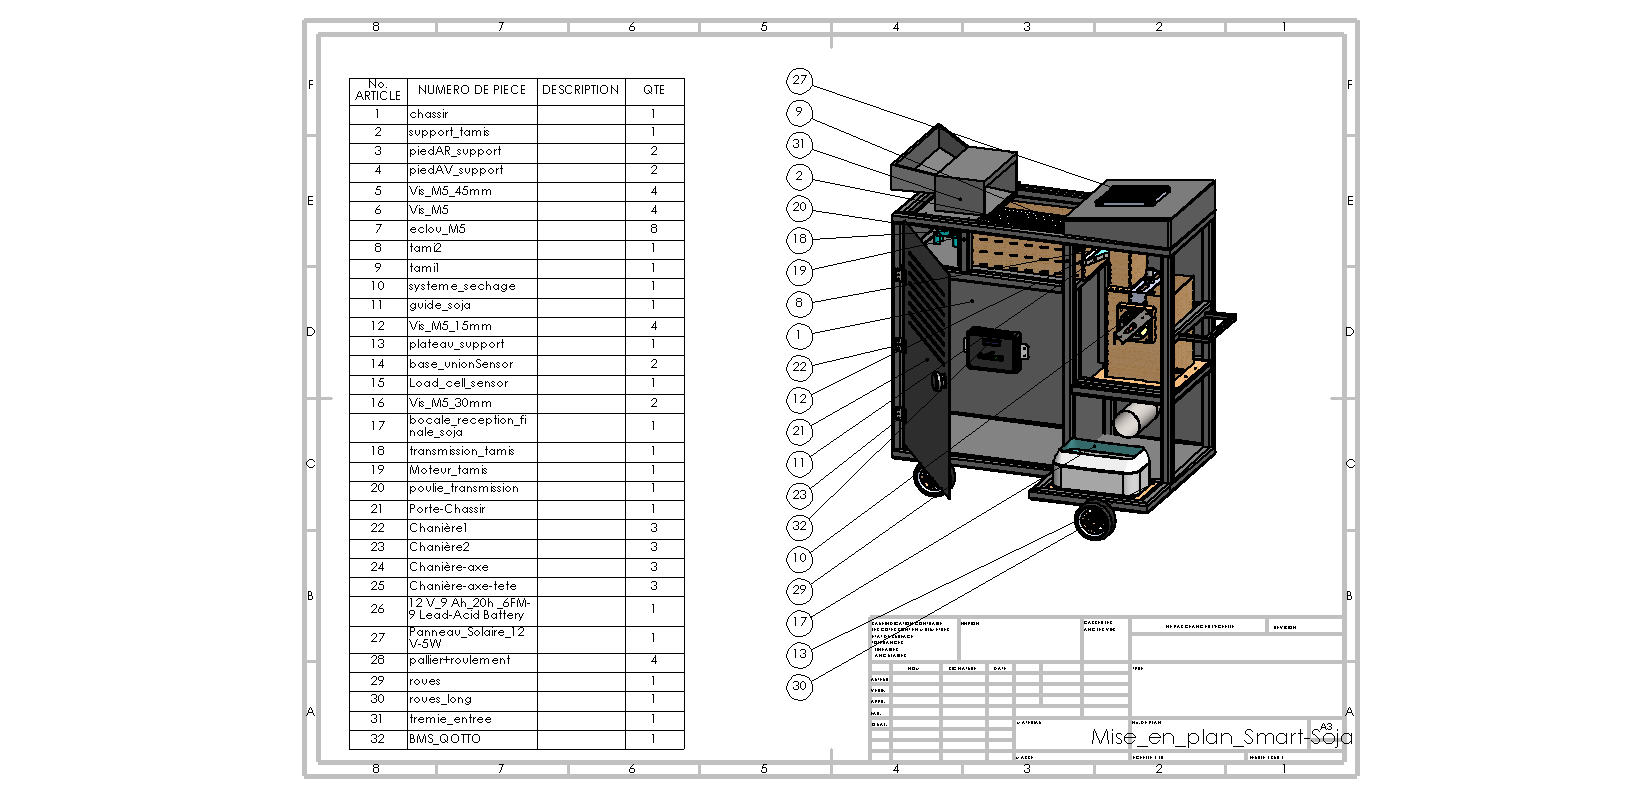
\includegraphics[width=\textwidth]{images/Mise_en_plan_Smart-Soja.PNG}
    \caption{Mise en plan technique et nomenclature (BOM) du châssis}
    \label{fig:mise_en_plan}
\end{figure}
\FloatBarrier

Chaque bloc peut être retiré du châssis sans démonter l'intégralité du système grâce à un système de glissières et connecteurs rapides — facteur clé pour la maintenance en milieu rural isolé.

\subsection{Fabrication et assemblage physique du châssis}
La phase de fabrication mécanique du châssis a nécessité la découpe de panneaux de contreplaqué haute densité aux dimensions précises de la modélisation SolidWorks. Cette opération a été réalisée à l'atelier de \textbf{Sèmè City Open Park} à l'aide d'une scie circulaire sur table (Figure~\ref{fig:decoupe_contreplaque}).

\begin{figure}[H]
    \centering
    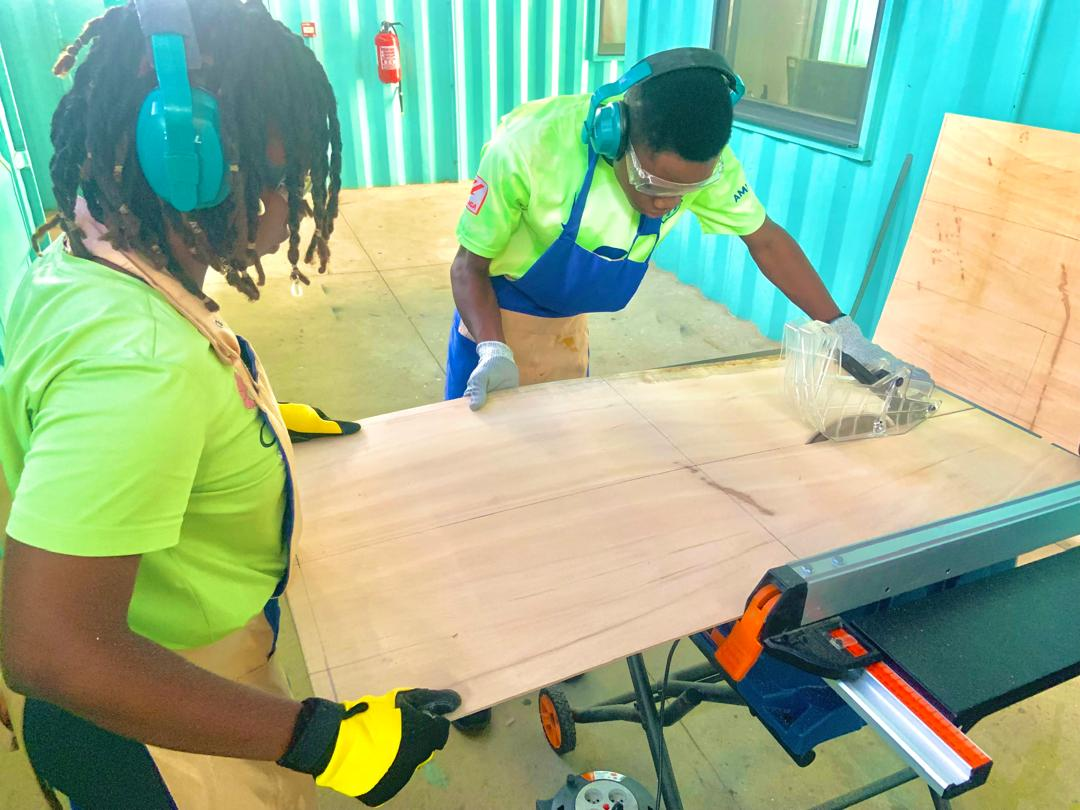
\includegraphics[width=0.55\textwidth]{images/decoupe_plaquet.jpg}
    \caption{Découpe du contreplaqué pour le châssis SMART-SOJA à Sèmè City Open Park}
    \label{fig:decoupe_contreplaque}
\end{figure}
\FloatBarrier

% -------------------------------------------------------
\section{Implémentation du firmware embarqué}
% -------------------------------------------------------
\label{sec:freertos_implementation}

\subsection{Architecture multitâches FreeRTOS}
Le firmware SMART-SOJA implémente \textbf{6 tâches FreeRTOS} ordonnancées selon leur criticité. La communication inter-tâches s'effectue via 5 files de messages (queues) pour un découplage robuste sans conditions de course (Tableau \ref{tab:freertos_tasks}).

\begin{table}[H]
    \caption{Hiérarchie des tâches FreeRTOS du firmware SMART-SOJA}
    \label{tab:freertos_tasks}
    \centering
    \small
    \renewcommand{\arraystretch}{1.8}
    \rowcolors{2}{white}{lightGray}
    \begin{tabularx}{\textwidth}{|L|>{\bfseries}C|C|L|}
        \hline
        \rowcolor{lightGray}
        \textbf{Tâche} & \textbf{Priorité} & \textbf{Cycle} & \textbf{Fonction} \\ \hline
        Task\_Safety    & 4 (MAX)  & 10 ms  & Arrêt d'urgence, surchauffe, timeout — temps réponse $<$ 10 ms. \\ \hline
        Task\_Control   & 3 (HIGH) & 50 ms  & Automate GRAFCET, gestion des transitions d'états. \\ \hline
        Task\_Sensing   & 2 (MED)  & 100 ms & Acquisition DHT22, Soil1/2, HX711 avec filtrage passe-bas. \\ \hline
        Task\_Actuators & 2 (MED)  & 50 ms  & Pilotage PWM moteurs, servo, LEDs. \\ \hline
        Task\_LCD       & 1 (LOW)  & 200 ms & Affichage I2C + lecture potentiomètres (ADC 0--4095 → 0--100\%). \\ \hline
        Task\_MQTT      & 1 (LOW)  & 500 ms & Transmission JSON, Store-and-Forward sur SD si déconnecté. \\ \hline
    \end{tabularx}
\end{table}
\FloatBarrier

Le flux de synchronisation entre tâches est illustré en Figure \ref{fig:arch_freertos} :

\begin{figure}[H]
    \centering
    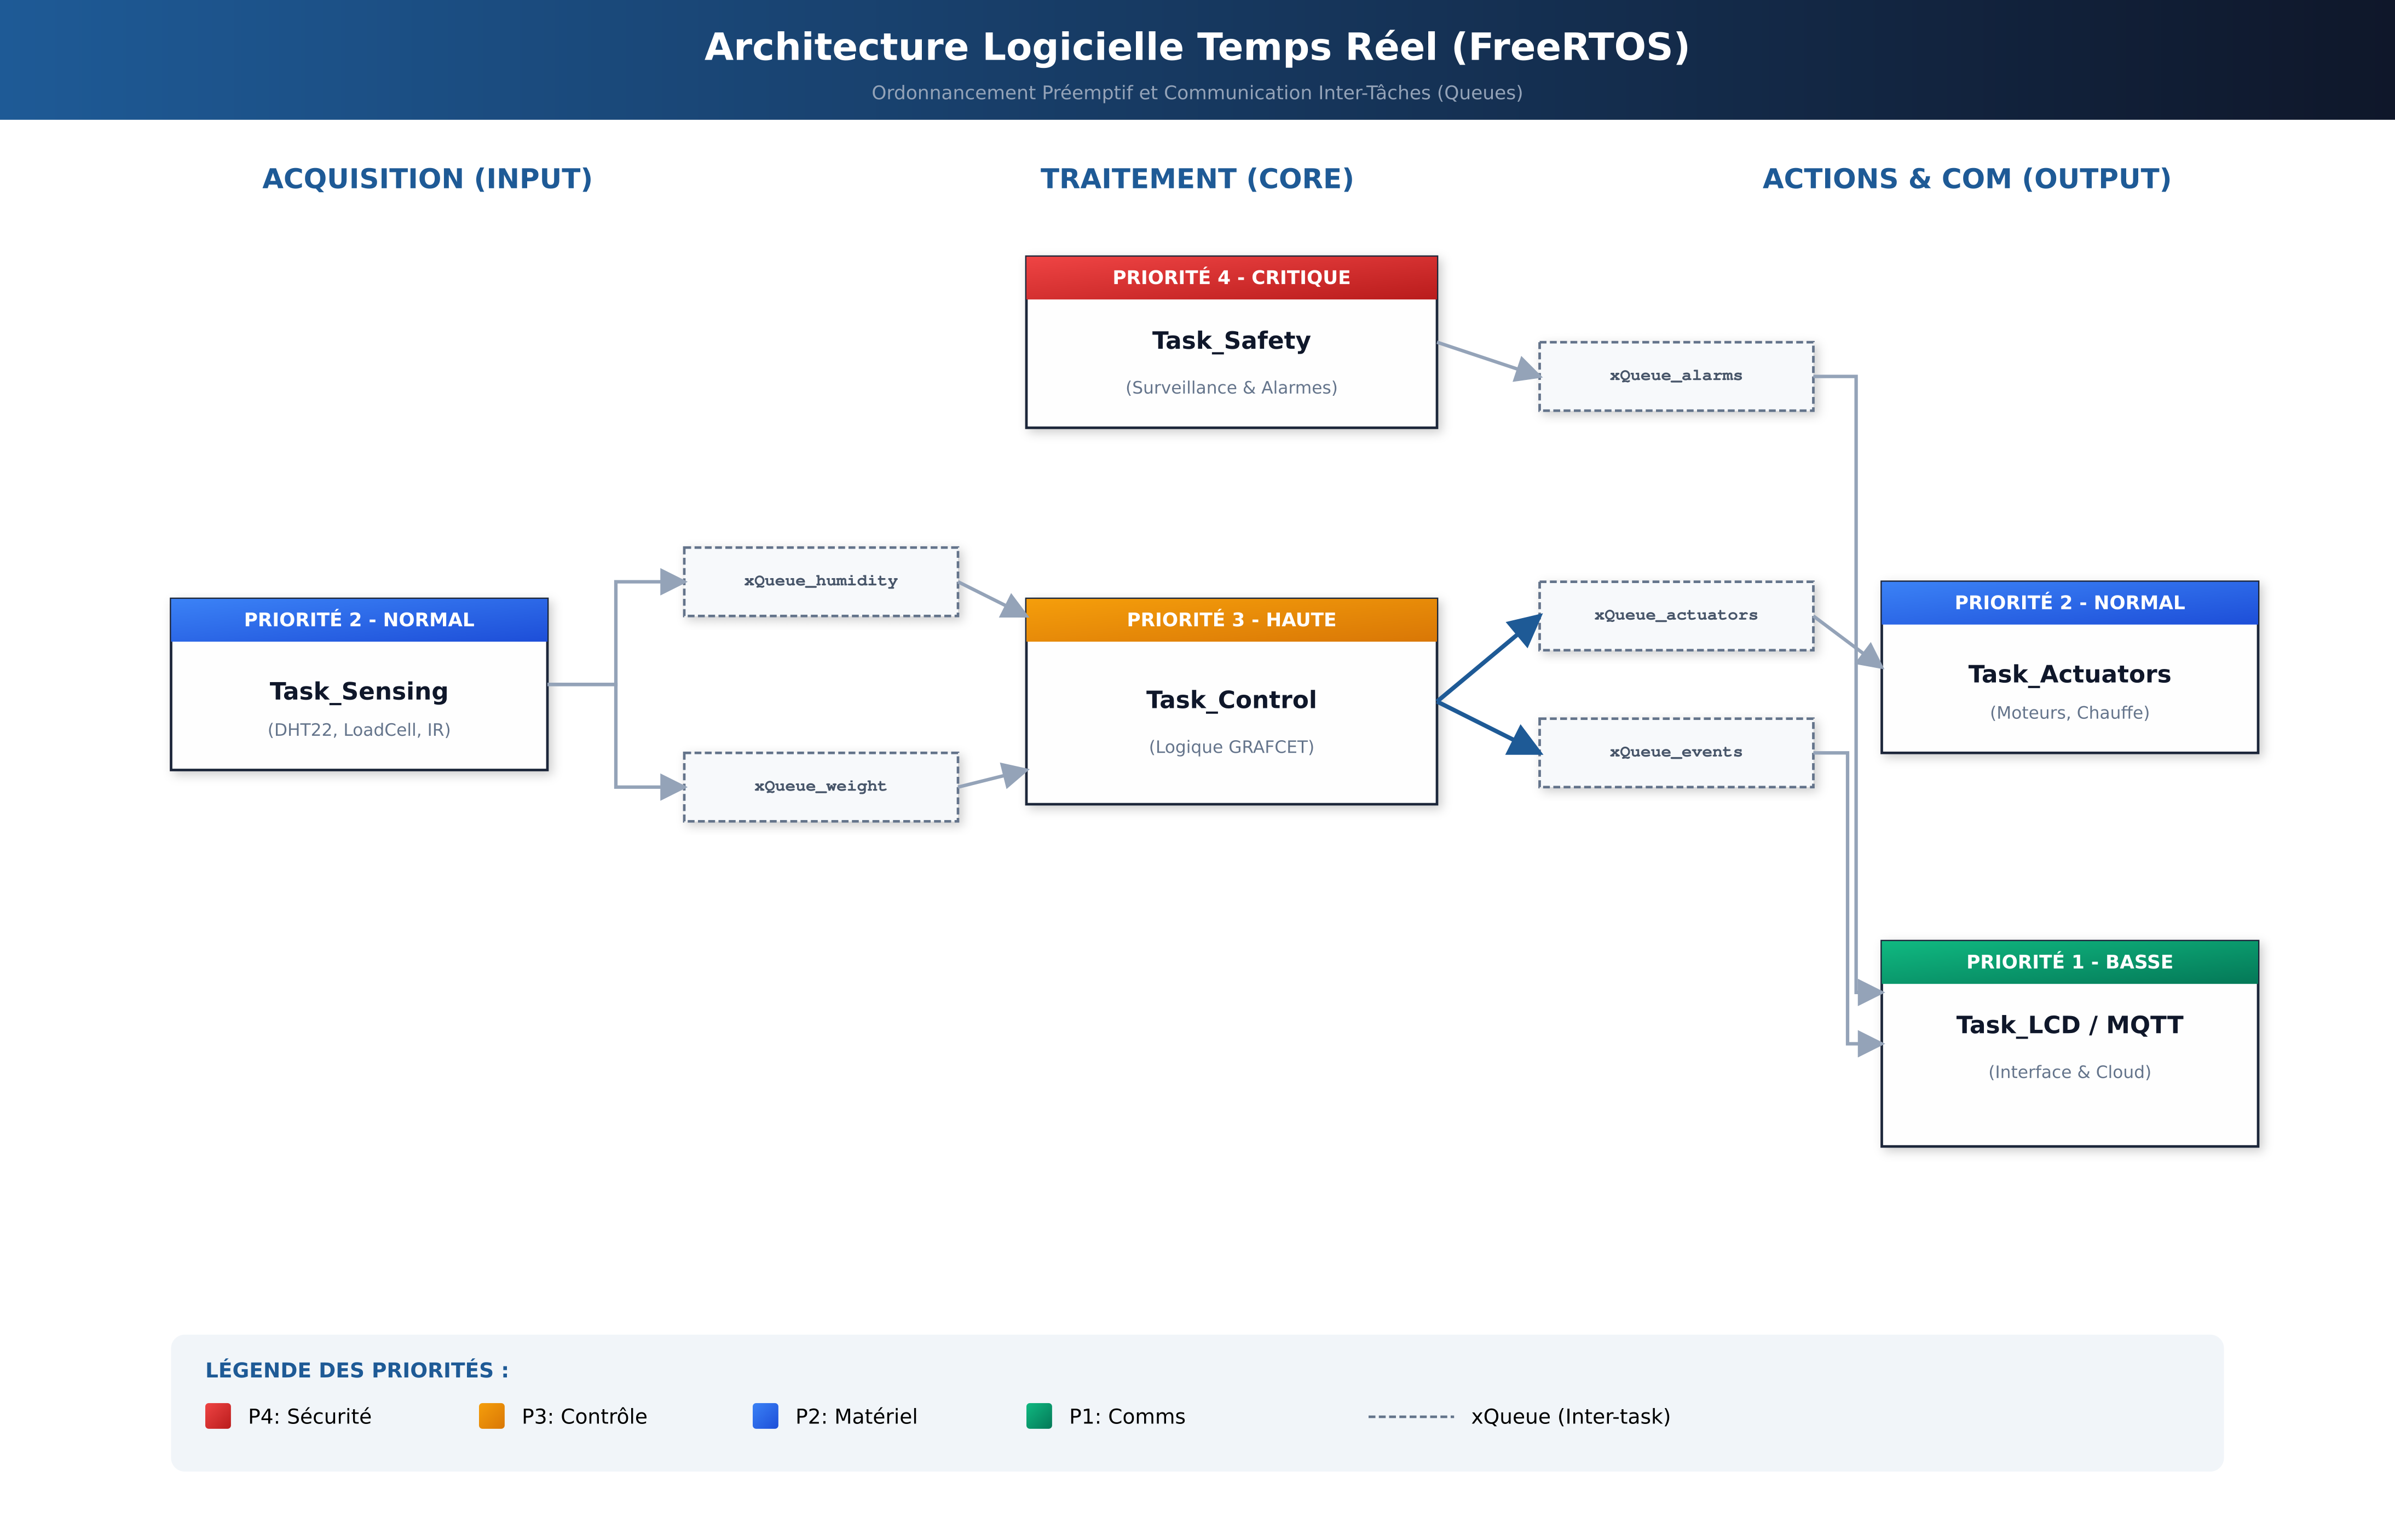
\includegraphics[width=\textwidth]{images/freertos_tasks.png}
    \caption{Diagramme de synchronisation des tâches FreeRTOS — SMART-SOJA}
    \label{fig:arch_freertos}
\end{figure}
\FloatBarrier

\subsection{Sérialisation et format de données (JSON)}
L'échange de données entre l'unité mobile ESP32 et la plateforme web de supervision s'effectue sous forme de messages sérialisés au format JSON. Deux types de trames sont principalement transmis :

\vspace{0.3cm}
\noindent\textbf{1. Trame de télémétrie périodique} (publiée toutes les 5~secondes sur le topic \texttt{smart-soja/telemetry/\{unitId\}}) : elle assure le suivi en temps réel de l'état de fonctionnement du prototype.
\begin{verbatim}
{
  "unitId": "SS-000110",
  "timestamp": 1716633600000,
  "humidity": 12.5,
  "temperature": 31.8,
  "weight": 42.3,
  "ir1": true,
  "ir2": false,
  "mode": "auto",
  "step": 3,
  "alarm": false,
  "controls": {
    "alimentation": false,
    "tamis": true,
    "ventilateur": false,
    "chauffage": true,
    "vis_soja": true,
    "servo_vanne": false
  },
  "battery": 95
}
\end{verbatim}

\vspace{0.3cm}
\noindent\textbf{2. Trame d'archivage de fin de cycle} (publiée sur le topic \texttt{smart-soja/lot\_completed/\{unitId\}} lors de la finalisation du traitement d'un lot) : elle certifie la qualité finale du soja.
\begin{verbatim}
{
  "unitId": "SS-000110",
  "timestamp": 1716633780000,
  "lotId": "LOT-TEST-002",
  "duration_ms": 180000,
  "weight_processed": 5000,
  "humidity_avg": 10.8,
  "temperature_avg": 31.8,
  "steps_completed": 12,
  "quality_score": 95
}
\end{verbatim}
\vspace{0.2cm}

Ce format de \textbf{passeport numérique} constitue la pièce centrale de la traçabilité Internet des objets : il lie chaque sac de soja à ses métriques de qualité certifiées, consultables depuis le tableau de bord web.

% -------------------------------------------------------
\section{Plateforme Internet des objets : tableau de bord de supervision}
% -------------------------------------------------------
La plateforme web \textbf{SMART-SOJA} constitue le centre de supervision et de traçabilité à distance du système. Elle a été développée selon une architecture de type \textbf{SPA} (\textit{Single Page Application}) en utilisant l'outillage moderne \textbf{Vite.js} et du \textbf{JavaScript (Vanilla JS)}. Ce choix garantit une interface utilisateur fluide, réactive et optimisée pour une consultation sur terminaux mobiles comme sur ordinateurs.

Le flux de données (Figure \ref{fig:diagram_mqtt}) repose sur un pipeline de communication bidirectionnel :
\begin{enumerate}
    \item \textbf{Collecte et Transport :} L'unité mobile publie les données de chaque lot au format JSON via le protocole \textbf{MQTT}.
    \item \textbf{Passerelle et Persistance :} Un serveur bridge sous \textbf{Node.js} intercepte ces messages pour les valider et les enregistrer instantanément dans la base de données temps réel \textbf{Firebase (Firestore)}.
    \item \textbf{Visualisation :} La plateforme web se synchronise automatiquement avec Firebase, permettant aux utilisateurs de suivre l'évolution de l'humidité et du poids des grains sans avoir à rafraîchir la page.
\end{enumerate}

\begin{figure}[H]
    \centering
    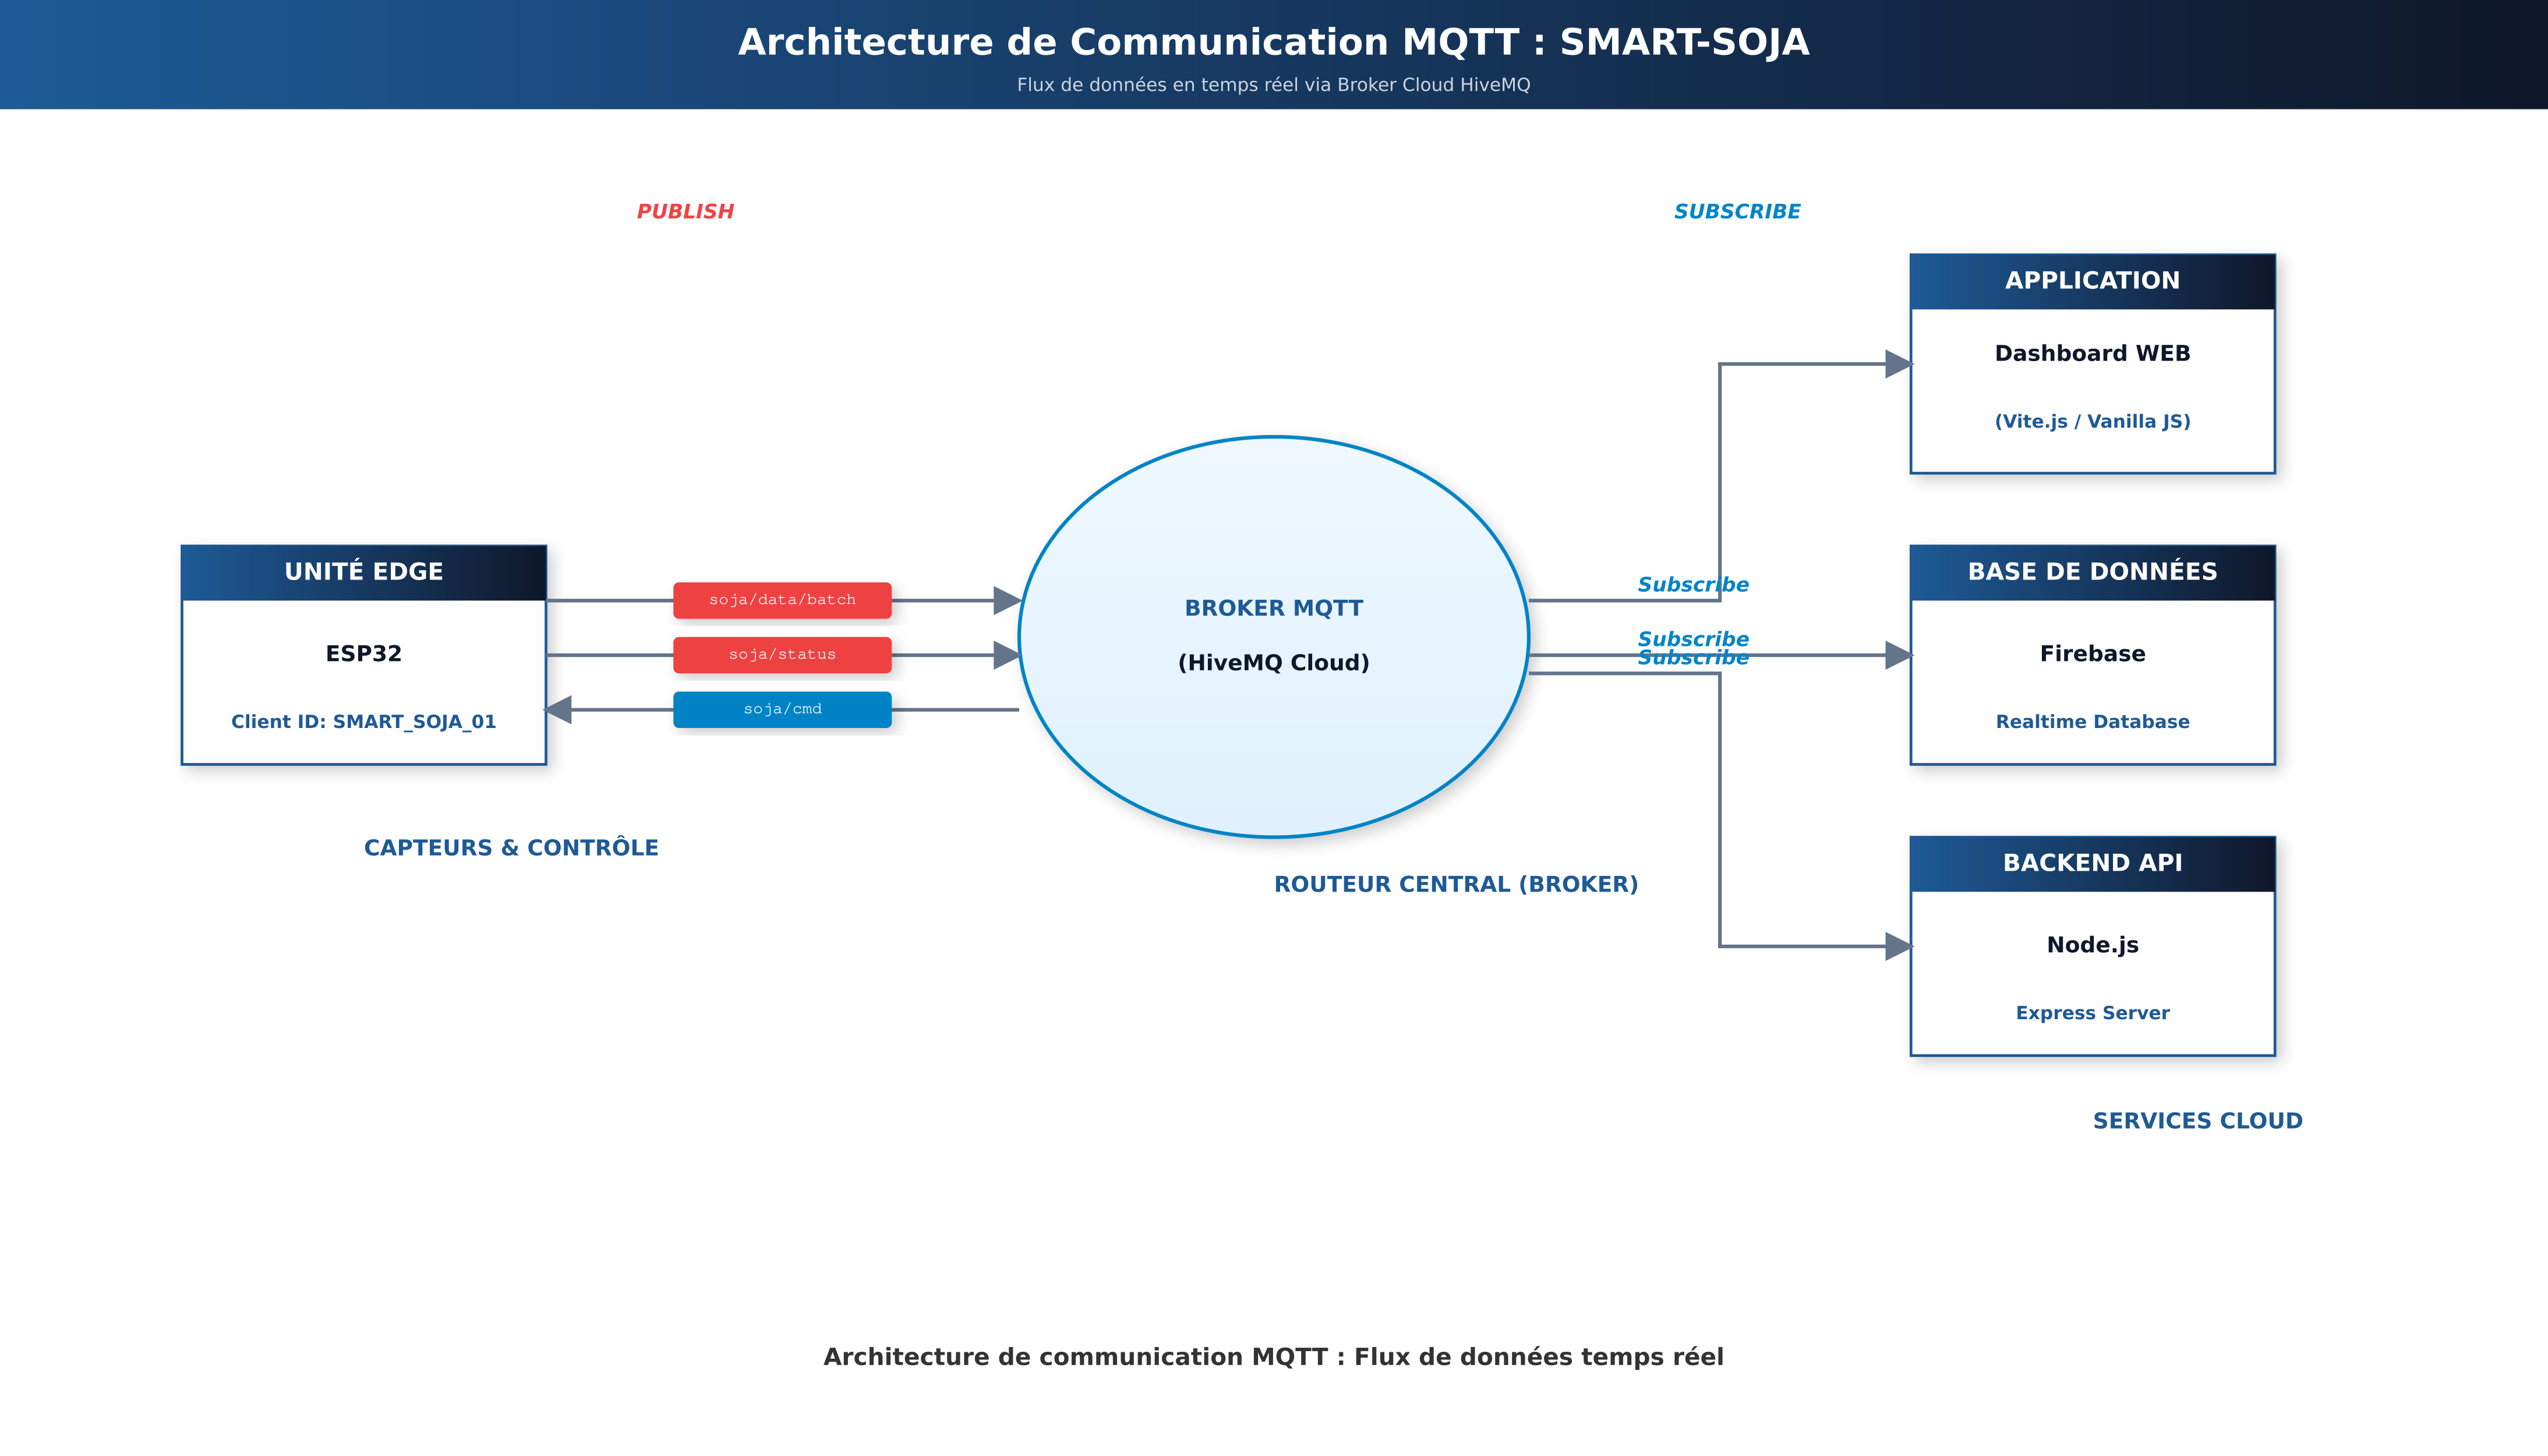
\includegraphics[width=\textwidth]{images/mqtt_architecture.png}
    \caption{Architecture de communication MQTT : Pipeline de données temps réel}
    \label{fig:diagram_mqtt}
\end{figure}
\FloatBarrier

Cette architecture garantit une \textbf{intégrité totale de la traçabilité} : chaque sac de soja possède son propre passeport numérique stocké de manière sécurisée dans le Cloud.

\begin{figure}[H]
    \centering
    \begin{subfigure}[b]{0.48\textwidth}
        \centering
        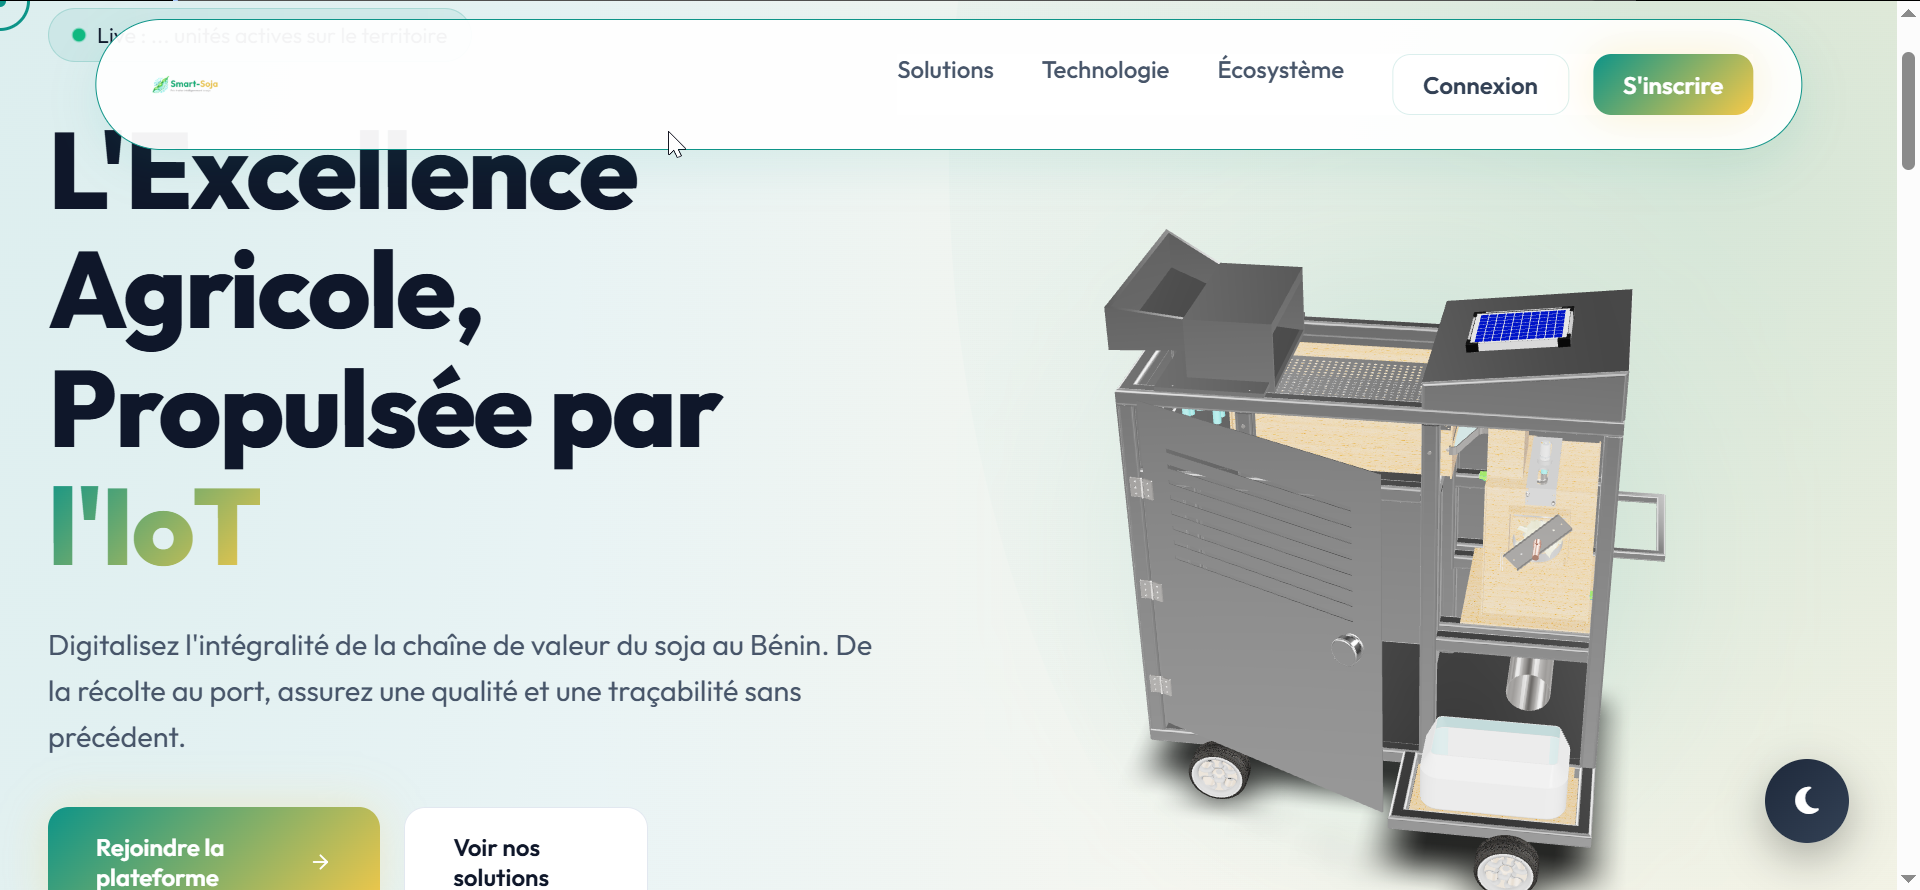
\includegraphics[width=\textwidth]{images/smart-soja-web_light.png}
        \caption{Mode Clair (\textit{Light Theme})}
    \end{subfigure}
    \hfill
    \begin{subfigure}[b]{0.48\textwidth}
        \centering
        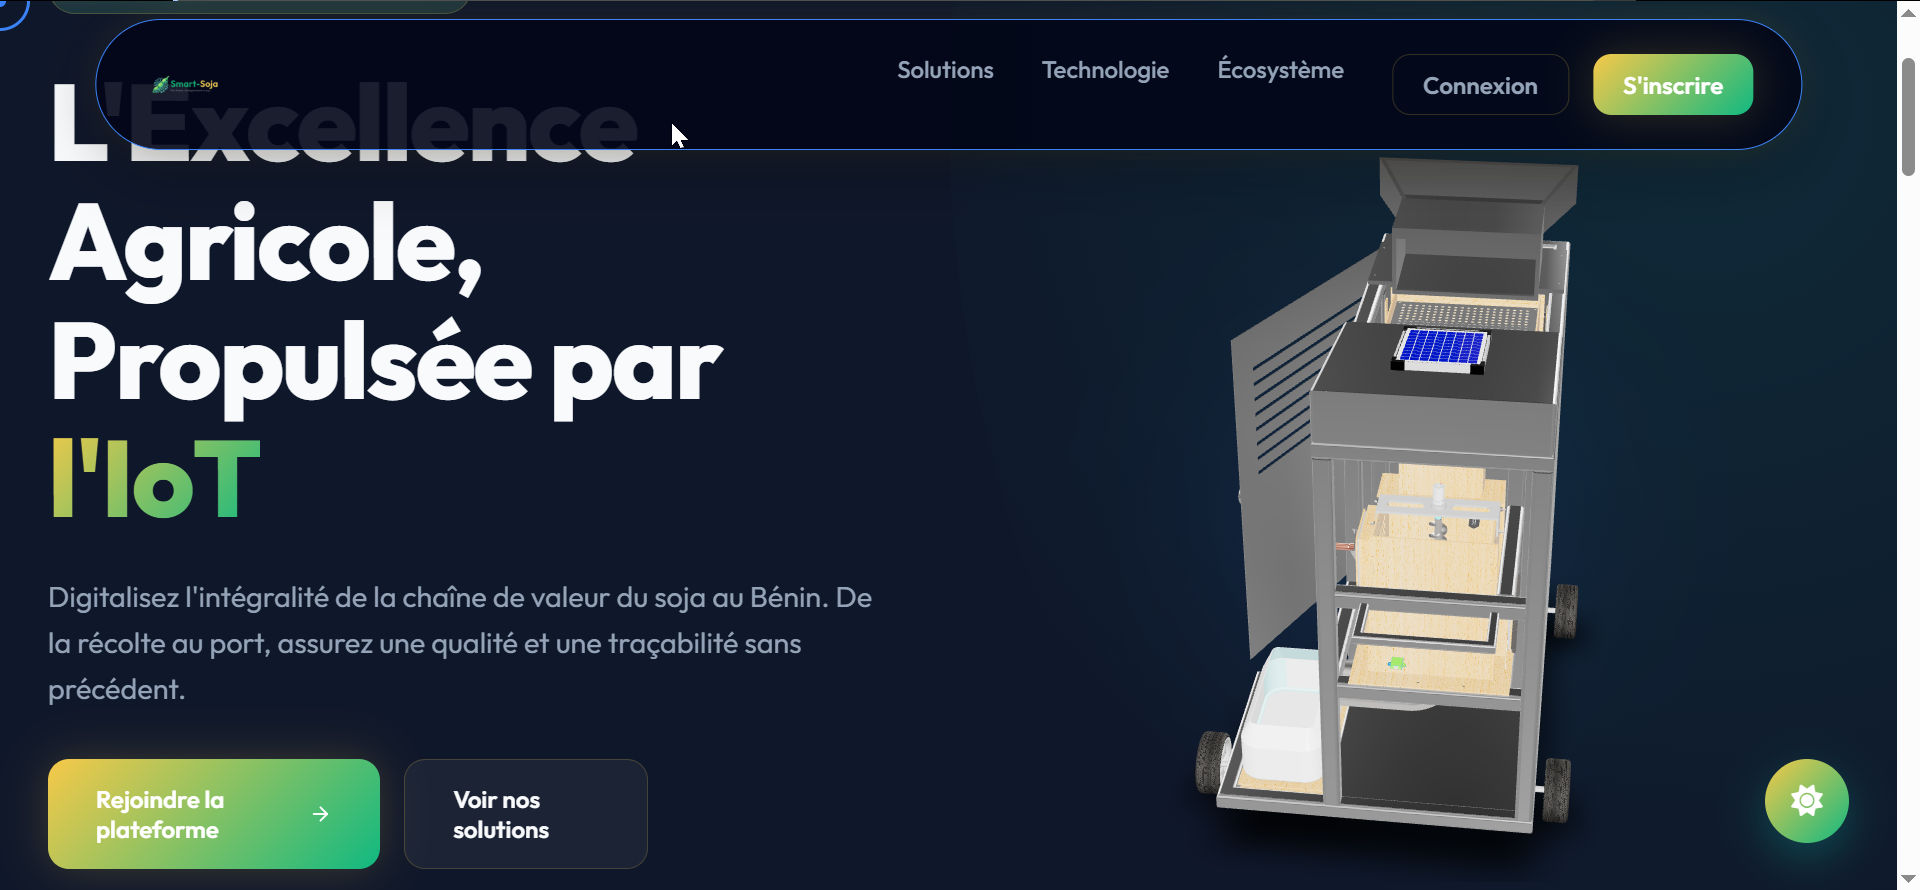
\includegraphics[width=\textwidth]{images/smart-soja-web_dark.png}
        \caption{Mode Sombre (\textit{Dark Theme})}
    \end{subfigure}
    \caption{Interface de présentation du projet SMART-SOJA — Page d'accueil (Vues multi-thèmes)}
    \label{fig:dashboard_themes}
\end{figure}
\FloatBarrier

Trois profils d'accès sont proposés :
\begin{itemize}
    \item \textbf{Tableau de bord Exploitant :} Suivi de production en temps réel, contrôle manuel des actionneurs via MQTT, alertes de maintenance.
    \item \textbf{Tableau de bord Industrie (GDIZ Ready) :} Validation de la qualité des lots entrants, graphiques d'humidité et température, impression des certificats de traçabilité PDF.
    \item \textbf{Tableau de bord Admin :} Gestion de la flotte de machines et des utilisateurs, audit système.
\end{itemize}

\FloatBarrier

% Fin de la section conception


\section*{Synthèse et transition}
Ce chapitre a présenté l'ensemble de la démarche de conception du système SMART-SOJA, depuis l'analyse du contexte de la filière soja au Bénin jusqu'à la réalisation concrète du prototype. L'architecture modulaire retenue, combinant mécanique, électronique, informatique embarquée et connectivité IoT, aboutit à un système cohérent et fonctionnel. Afin de valider la viabilité de cette solution mécatronique et de vérifier sa conformité au cahier des charges fonctionnel sous des contraintes réelles, une série d'essais expérimentaux a été menée sur le site de QOTTO Bénin. Les résultats quantitatifs de cette phase d'évaluation des performances, ainsi que leur analyse critique et les discussions associées, font l'objet du chapitre suivant.
